\documentclass[twoside]{book}

% Packages required by doxygen
\usepackage{fixltx2e}
\usepackage{calc}
\usepackage{doxygen}
\usepackage[export]{adjustbox} % also loads graphicx
\usepackage{graphicx}
\usepackage[utf8]{inputenc}
\usepackage{makeidx}
\usepackage{multicol}
\usepackage{multirow}
\PassOptionsToPackage{warn}{textcomp}
\usepackage{textcomp}
\usepackage[nointegrals]{wasysym}
\usepackage[table]{xcolor}

% Font selection
\usepackage[T1]{fontenc}
\usepackage[scaled=.90]{helvet}
\usepackage{courier}
\usepackage{amssymb}
\usepackage{sectsty}
\renewcommand{\familydefault}{\sfdefault}
\allsectionsfont{%
  \fontseries{bc}\selectfont%
  \color{darkgray}%
}
\renewcommand{\DoxyLabelFont}{%
  \fontseries{bc}\selectfont%
  \color{darkgray}%
}
\newcommand{\+}{\discretionary{\mbox{\scriptsize$\hookleftarrow$}}{}{}}

% Page & text layout
\usepackage{geometry}
\geometry{%
  a4paper,%
  top=2.5cm,%
  bottom=2.5cm,%
  left=2.5cm,%
  right=2.5cm%
}
\tolerance=750
\hfuzz=15pt
\hbadness=750
\setlength{\emergencystretch}{15pt}
\setlength{\parindent}{0cm}
\setlength{\parskip}{3ex plus 2ex minus 2ex}
\makeatletter
\renewcommand{\paragraph}{%
  \@startsection{paragraph}{4}{0ex}{-1.0ex}{1.0ex}{%
    \normalfont\normalsize\bfseries\SS@parafont%
  }%
}
\renewcommand{\subparagraph}{%
  \@startsection{subparagraph}{5}{0ex}{-1.0ex}{1.0ex}{%
    \normalfont\normalsize\bfseries\SS@subparafont%
  }%
}
\makeatother

% Headers & footers
\usepackage{fancyhdr}
\pagestyle{fancyplain}
\fancyhead[LE]{\fancyplain{}{\bfseries\thepage}}
\fancyhead[CE]{\fancyplain{}{}}
\fancyhead[RE]{\fancyplain{}{\bfseries\leftmark}}
\fancyhead[LO]{\fancyplain{}{\bfseries\rightmark}}
\fancyhead[CO]{\fancyplain{}{}}
\fancyhead[RO]{\fancyplain{}{\bfseries\thepage}}
\fancyfoot[LE]{\fancyplain{}{}}
\fancyfoot[CE]{\fancyplain{}{}}
\fancyfoot[RE]{\fancyplain{}{\bfseries\scriptsize Generated by Doxygen }}
\fancyfoot[LO]{\fancyplain{}{\bfseries\scriptsize Generated by Doxygen }}
\fancyfoot[CO]{\fancyplain{}{}}
\fancyfoot[RO]{\fancyplain{}{}}
\renewcommand{\footrulewidth}{0.4pt}
\renewcommand{\chaptermark}[1]{%
  \markboth{#1}{}%
}
\renewcommand{\sectionmark}[1]{%
  \markright{\thesection\ #1}%
}

% Indices & bibliography
\usepackage{natbib}
\usepackage[titles]{tocloft}
\setcounter{tocdepth}{3}
\setcounter{secnumdepth}{5}
\makeindex

% Hyperlinks (required, but should be loaded last)
\usepackage{ifpdf}
\ifpdf
  \usepackage[pdftex,pagebackref=true]{hyperref}
\else
  \usepackage[ps2pdf,pagebackref=true]{hyperref}
\fi
\hypersetup{%
  colorlinks=true,%
  linkcolor=blue,%
  citecolor=blue,%
  unicode%
}

% Custom commands
\newcommand{\clearemptydoublepage}{%
  \newpage{\pagestyle{empty}\cleardoublepage}%
}

\usepackage{caption}
\captionsetup{labelsep=space,justification=centering,font={bf},singlelinecheck=off,skip=4pt,position=top}

%===== C O N T E N T S =====

\begin{document}

% Titlepage & ToC
\hypersetup{pageanchor=false,
             bookmarksnumbered=true,
             pdfencoding=unicode
            }
\pagenumbering{roman}
\begin{titlepage}
\vspace*{7cm}
\begin{center}%
{\Large My Project \\[1ex]\large ff }\\
\vspace*{1cm}
{\large Generated by Doxygen 1.8.11}\\
\end{center}
\end{titlepage}
\clearemptydoublepage
\tableofcontents
\clearemptydoublepage
\pagenumbering{arabic}
\hypersetup{pageanchor=true}

%--- Begin generated contents ---
\chapter{Lightbox2}
\label{md_home_Galeria_lightbox_README}
\hypertarget{md_home_Galeria_lightbox_README}{}
by Lokesh Dhakar $\vert$ \href{http://www.lokeshdhakar.com}{\tt lokeshdhakar.\+com} $\vert$ \href{http://twitter.com/lokeshdhakar}{\tt twitter.\+com/lokeshdhakar}

For more information\+: \href{http://lokeshdhakar.com/projects/lightbox2/}{\tt http\+://lokeshdhakar.\+com/projects/lightbox2/} 
\chapter{Namespace Index}
\section{Packages}
Here are the packages with brief descriptions (if available)\+:\begin{DoxyCompactList}
\item\contentsline{section}{\hyperlink{namespace_sica_segura}{Sica\+Segura} }{\pageref{namespace_sica_segura}}{}
\end{DoxyCompactList}

\chapter{Hierarchical Index}
\section{Class Hierarchy}
This inheritance list is sorted roughly, but not completely, alphabetically\+:\begin{DoxyCompactList}
\item \contentsline{section}{Sica\+Segura.\+S\+I\+C\+A\+\_\+\+Punto\+Control.\+Lectura}{\pageref{class_sica_segura_1_1_s_i_c_a___punto_control_1_1_lectura}}{}
\item Page\begin{DoxyCompactList}
\item \contentsline{section}{download}{\pageref{classdownload}}{}
\item \contentsline{section}{librodigital\+\_\+home\+\_\+\+Borrar\+Punto\+Sesion}{\pageref{classlibrodigital__home___borrar_punto_sesion}}{}
\item \contentsline{section}{librodigital\+\_\+home\+\_\+\+Borrar\+Punto\+Sesion}{\pageref{classlibrodigital__home___borrar_punto_sesion}}{}
\item \contentsline{section}{librodigital\+\_\+home\+\_\+index}{\pageref{classlibrodigital__home__index}}{}
\item \contentsline{section}{librodigital\+\_\+home\+\_\+\+Inf\+Adm}{\pageref{classlibrodigital__home___inf_adm}}{}
\item \contentsline{section}{librodigital\+\_\+home\+\_\+\+Inf\+Geografica}{\pageref{classlibrodigital__home___inf_geografica}}{}
\item \contentsline{section}{librodigital\+\_\+home\+\_\+\+Info\+Usuario}{\pageref{classlibrodigital__home___info_usuario}}{}
\item \contentsline{section}{librodigital\+\_\+home\+\_\+\+Nuevalectura}{\pageref{classlibrodigital__home___nuevalectura}}{}
\item \contentsline{section}{S\+I\+C\+A\+H\+\_\+\+Galeria\+\_\+galeria}{\pageref{class_s_i_c_a_h___galeria__galeria}}{}
\item \contentsline{section}{S\+I\+C\+A\+H\+\_\+\+Galeria\+\_\+galeria}{\pageref{class_s_i_c_a_h___galeria__galeria}}{}
\end{DoxyCompactList}
\item \contentsline{section}{Sica\+Segura.\+S\+I\+C\+A\+\_\+\+Agrupacion}{\pageref{class_sica_segura_1_1_s_i_c_a___agrupacion}}{}
\item \contentsline{section}{Sica\+Segura.\+S\+I\+C\+A\+\_\+\+DB}{\pageref{class_sica_segura_1_1_s_i_c_a___d_b}}{}
\item \contentsline{section}{Sica\+Segura.\+S\+I\+C\+A\+\_\+\+Libro\+Control}{\pageref{class_sica_segura_1_1_s_i_c_a___libro_control}}{}
\item \contentsline{section}{Sica\+Segura.\+S\+I\+C\+A\+\_\+\+Log}{\pageref{class_sica_segura_1_1_s_i_c_a___log}}{}
\item \contentsline{section}{Sica\+Segura.\+S\+I\+C\+A\+\_\+\+Punto\+Control}{\pageref{class_sica_segura_1_1_s_i_c_a___punto_control}}{}
\item \contentsline{section}{Sica\+Segura.\+S\+I\+C\+A\+\_\+\+Sysem\+IO}{\pageref{class_sica_segura_1_1_s_i_c_a___sysem_i_o}}{}
\end{DoxyCompactList}

\chapter{Class Index}
\section{Class List}
Here are the classes, structs, unions and interfaces with brief descriptions\+:\begin{DoxyCompactList}
\item\contentsline{section}{\hyperlink{classdownload}{download} }{\pageref{classdownload}}{}
\item\contentsline{section}{\hyperlink{class_sica_segura_1_1_s_i_c_a___punto_control_1_1_lectura}{Sica\+Segura.\+S\+I\+C\+A\+\_\+\+Punto\+Control.\+Lectura} }{\pageref{class_sica_segura_1_1_s_i_c_a___punto_control_1_1_lectura}}{}
\item\contentsline{section}{\hyperlink{classlibrodigital__home___borrar_punto_sesion}{librodigital\+\_\+home\+\_\+\+Borrar\+Punto\+Sesion} }{\pageref{classlibrodigital__home___borrar_punto_sesion}}{}
\item\contentsline{section}{\hyperlink{classlibrodigital__home__index}{librodigital\+\_\+home\+\_\+index} }{\pageref{classlibrodigital__home__index}}{}
\item\contentsline{section}{\hyperlink{classlibrodigital__home___inf_adm}{librodigital\+\_\+home\+\_\+\+Inf\+Adm} }{\pageref{classlibrodigital__home___inf_adm}}{}
\item\contentsline{section}{\hyperlink{classlibrodigital__home___inf_geografica}{librodigital\+\_\+home\+\_\+\+Inf\+Geografica} }{\pageref{classlibrodigital__home___inf_geografica}}{}
\item\contentsline{section}{\hyperlink{classlibrodigital__home___info_usuario}{librodigital\+\_\+home\+\_\+\+Info\+Usuario} }{\pageref{classlibrodigital__home___info_usuario}}{}
\item\contentsline{section}{\hyperlink{classlibrodigital__home___nuevalectura}{librodigital\+\_\+home\+\_\+\+Nuevalectura} }{\pageref{classlibrodigital__home___nuevalectura}}{}
\item\contentsline{section}{\hyperlink{class_sica_segura_1_1_s_i_c_a___agrupacion}{Sica\+Segura.\+S\+I\+C\+A\+\_\+\+Agrupacion} }{\pageref{class_sica_segura_1_1_s_i_c_a___agrupacion}}{}
\item\contentsline{section}{\hyperlink{class_sica_segura_1_1_s_i_c_a___d_b}{Sica\+Segura.\+S\+I\+C\+A\+\_\+\+DB} }{\pageref{class_sica_segura_1_1_s_i_c_a___d_b}}{}
\item\contentsline{section}{\hyperlink{class_sica_segura_1_1_s_i_c_a___libro_control}{Sica\+Segura.\+S\+I\+C\+A\+\_\+\+Libro\+Control} }{\pageref{class_sica_segura_1_1_s_i_c_a___libro_control}}{}
\item\contentsline{section}{\hyperlink{class_sica_segura_1_1_s_i_c_a___log}{Sica\+Segura.\+S\+I\+C\+A\+\_\+\+Log} \\*Clase cuya función es la de registrar los movimientos realizados en la Web. }{\pageref{class_sica_segura_1_1_s_i_c_a___log}}{}
\item\contentsline{section}{\hyperlink{class_sica_segura_1_1_s_i_c_a___punto_control}{Sica\+Segura.\+S\+I\+C\+A\+\_\+\+Punto\+Control} }{\pageref{class_sica_segura_1_1_s_i_c_a___punto_control}}{}
\item\contentsline{section}{\hyperlink{class_sica_segura_1_1_s_i_c_a___sysem_i_o}{Sica\+Segura.\+S\+I\+C\+A\+\_\+\+Sysem\+IO} }{\pageref{class_sica_segura_1_1_s_i_c_a___sysem_i_o}}{}
\item\contentsline{section}{\hyperlink{class_s_i_c_a_h___galeria__galeria}{S\+I\+C\+A\+H\+\_\+\+Galeria\+\_\+galeria} }{\pageref{class_s_i_c_a_h___galeria__galeria}}{}
\end{DoxyCompactList}

\chapter{Namespace Documentation}
\hypertarget{namespace_sica_segura}{}\section{Sica\+Segura Namespace Reference}
\label{namespace_sica_segura}\index{Sica\+Segura@{Sica\+Segura}}
\subsection*{Classes}
\begin{DoxyCompactItemize}
\item 
class \hyperlink{class_sica_segura_1_1_s_i_c_a___agrupacion}{S\+I\+C\+A\+\_\+\+Agrupacion}
\item 
class \hyperlink{class_sica_segura_1_1_s_i_c_a___d_b}{S\+I\+C\+A\+\_\+\+DB}
\item 
class \hyperlink{class_sica_segura_1_1_s_i_c_a___libro_control}{S\+I\+C\+A\+\_\+\+Libro\+Control}
\item 
class \hyperlink{class_sica_segura_1_1_s_i_c_a___log}{S\+I\+C\+A\+\_\+\+Log}
\begin{DoxyCompactList}\small\item\em Clase cuya función es la de registrar los movimientos realizados en la Web. \end{DoxyCompactList}\item 
class \hyperlink{class_sica_segura_1_1_s_i_c_a___punto_control}{S\+I\+C\+A\+\_\+\+Punto\+Control}
\item 
class \hyperlink{class_sica_segura_1_1_s_i_c_a___sysem_i_o}{S\+I\+C\+A\+\_\+\+Sysem\+IO}
\end{DoxyCompactItemize}

\chapter{Class Documentation}
\hypertarget{classdownload}{}\section{download Class Reference}
\label{classdownload}\index{download@{download}}
Inheritance diagram for download\+:\begin{figure}[H]
\begin{center}
\leavevmode
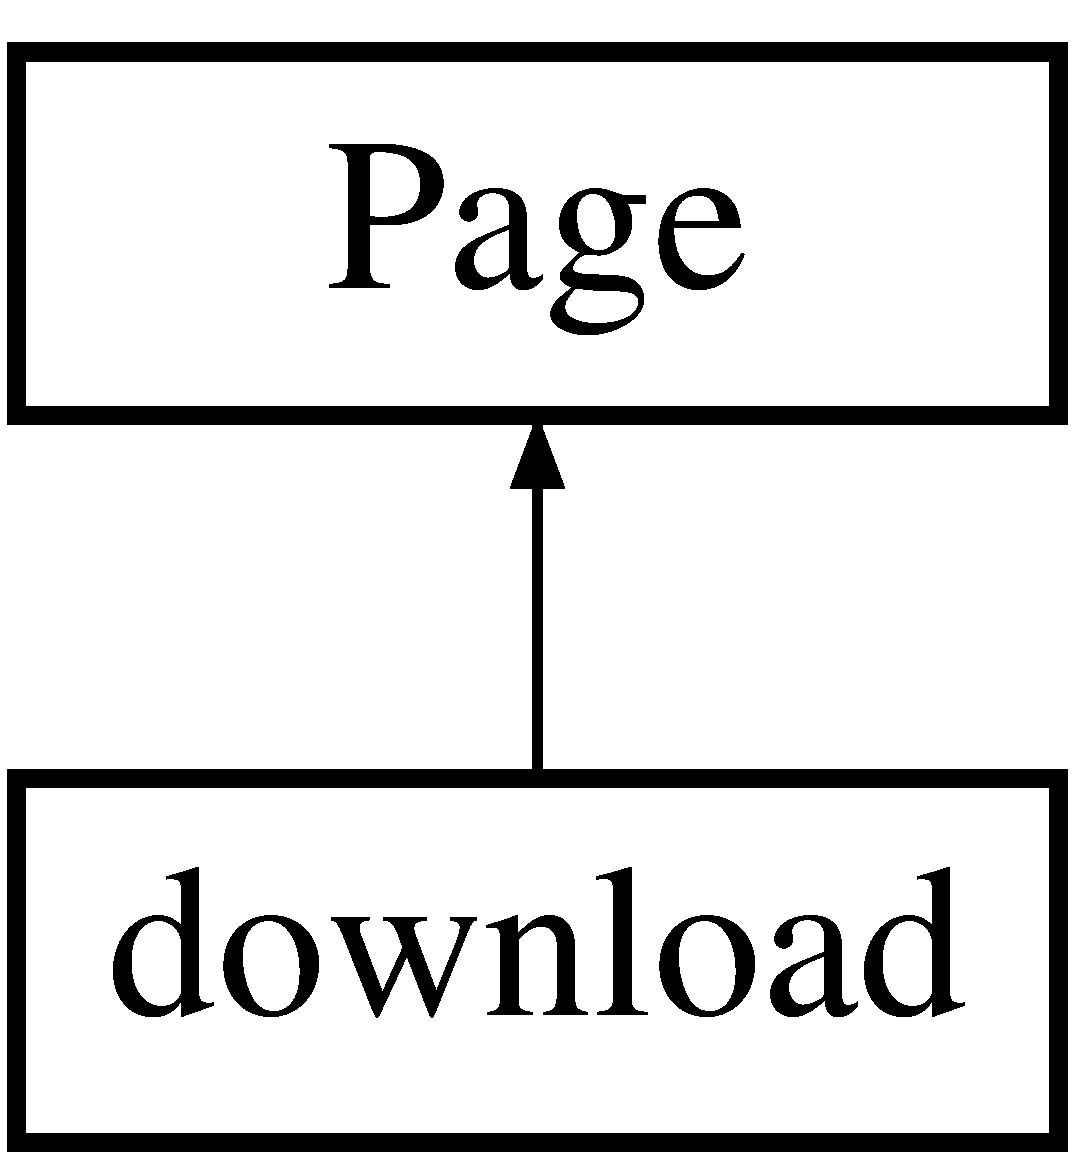
\includegraphics[height=2.000000cm]{classdownload}
\end{center}
\end{figure}
\subsection*{Protected Member Functions}
\begin{DoxyCompactItemize}
\item 
void \hyperlink{classdownload_a1fd4257623e49112f1d72043b456e11b}{Page\+\_\+\+Load} (object sender, Event\+Args e)
\end{DoxyCompactItemize}
\subsection*{Private Member Functions}
\begin{DoxyCompactItemize}
\item 
void \hyperlink{classdownload_a40d8a7337768a2ab91fcc430f35a6f27}{Transmit\+File} (Http\+Context context, string file\+Path, string download\+Name, bool force\+Download)
\begin{DoxyCompactList}\small\item\em Funcion desarrollada para realizar a modo de \char`\"{}black\+Box\char`\"{} la descarga de los ficheros Cualquier documento para la descarga se encuentra en una ruta no pública a la que accede la aplicación web para la descarga. El fichero se lee y se devuelve al usuario como un fichero nuevo con el formato y contenido del que se encuentra en el servidor. \end{DoxyCompactList}\end{DoxyCompactItemize}


\subsection{Detailed Description}


Definition at line 12 of file download.\+aspx.\+cs.



\subsection{Member Function Documentation}
\index{download@{download}!Page\+\_\+\+Load@{Page\+\_\+\+Load}}
\index{Page\+\_\+\+Load@{Page\+\_\+\+Load}!download@{download}}
\subsubsection[{\texorpdfstring{Page\+\_\+\+Load(object sender, Event\+Args e)}{Page_Load(object sender, EventArgs e)}}]{\setlength{\rightskip}{0pt plus 5cm}void download.\+Page\+\_\+\+Load (
\begin{DoxyParamCaption}
\item[{object}]{sender, }
\item[{Event\+Args}]{e}
\end{DoxyParamCaption}
)\hspace{0.3cm}{\ttfamily [protected]}}\hypertarget{classdownload_a1fd4257623e49112f1d72043b456e11b}{}\label{classdownload_a1fd4257623e49112f1d72043b456e11b}
Comprobamos que se ha pasado por la página indexcas.\+aspx y se ha hecho login 

Definition at line 14 of file download.\+aspx.\+cs.

\index{download@{download}!Transmit\+File@{Transmit\+File}}
\index{Transmit\+File@{Transmit\+File}!download@{download}}
\subsubsection[{\texorpdfstring{Transmit\+File(\+Http\+Context context, string file\+Path, string download\+Name, bool force\+Download)}{TransmitFile(HttpContext context, string filePath, string downloadName, bool forceDownload)}}]{\setlength{\rightskip}{0pt plus 5cm}void download.\+Transmit\+File (
\begin{DoxyParamCaption}
\item[{Http\+Context}]{context, }
\item[{string}]{file\+Path, }
\item[{string}]{download\+Name, }
\item[{bool}]{force\+Download}
\end{DoxyParamCaption}
)\hspace{0.3cm}{\ttfamily [private]}}\hypertarget{classdownload_a40d8a7337768a2ab91fcc430f35a6f27}{}\label{classdownload_a40d8a7337768a2ab91fcc430f35a6f27}


Funcion desarrollada para realizar a modo de \char`\"{}black\+Box\char`\"{} la descarga de los ficheros Cualquier documento para la descarga se encuentra en una ruta no pública a la que accede la aplicación web para la descarga. El fichero se lee y se devuelve al usuario como un fichero nuevo con el formato y contenido del que se encuentra en el servidor. 


\begin{DoxyParams}{Parameters}
{\em context} & Http\+Context\\
\hline
{\em file\+Path} & Ruta Absoluta del fichero a descargar\\
\hline
{\em download\+Name} & Nombre con el que se descargará el fichero\\
\hline
{\em force\+Download} & Permite que la descarga se incruste en el navegador o siempre se descargue\\
\hline
\end{DoxyParams}


Definition at line 57 of file download.\+aspx.\+cs.



The documentation for this class was generated from the following file\+:\begin{DoxyCompactItemize}
\item 
home/download.\+aspx.\+cs\end{DoxyCompactItemize}

\hypertarget{class_sica_segura_1_1_s_i_c_a___punto_control_1_1_lectura}{}\section{Sica\+Segura.\+S\+I\+C\+A\+\_\+\+Punto\+Control.\+Lectura Class Reference}
\label{class_sica_segura_1_1_s_i_c_a___punto_control_1_1_lectura}\index{Sica\+Segura.\+S\+I\+C\+A\+\_\+\+Punto\+Control.\+Lectura@{Sica\+Segura.\+S\+I\+C\+A\+\_\+\+Punto\+Control.\+Lectura}}
\subsection*{Public Member Functions}
\begin{DoxyCompactItemize}
\item 
{\bfseries Lectura} (Date\+Time fecha, double lectura)\hypertarget{class_sica_segura_1_1_s_i_c_a___punto_control_1_1_lectura_a812404e74ae64212ff661114d2af8c69}{}\label{class_sica_segura_1_1_s_i_c_a___punto_control_1_1_lectura_a812404e74ae64212ff661114d2af8c69}

\item 
Date\+Time {\bfseries Get\+\_\+\+Fecha\+\_\+\+Medida} ()\hypertarget{class_sica_segura_1_1_s_i_c_a___punto_control_1_1_lectura_af4aadae0a9aefdfe5ceb709079073bb9}{}\label{class_sica_segura_1_1_s_i_c_a___punto_control_1_1_lectura_af4aadae0a9aefdfe5ceb709079073bb9}

\item 
double {\bfseries Get\+\_\+valor} ()\hypertarget{class_sica_segura_1_1_s_i_c_a___punto_control_1_1_lectura_a32f8cc98764a878a1bcbe92b71ed74ea}{}\label{class_sica_segura_1_1_s_i_c_a___punto_control_1_1_lectura_a32f8cc98764a878a1bcbe92b71ed74ea}

\end{DoxyCompactItemize}
\subsection*{Private Attributes}
\begin{DoxyCompactItemize}
\item 
Date\+Time {\bfseries fecha\+\_\+medida}\hypertarget{class_sica_segura_1_1_s_i_c_a___punto_control_1_1_lectura_a983e701c7bf6a75f8d79b37330ac11d6}{}\label{class_sica_segura_1_1_s_i_c_a___punto_control_1_1_lectura_a983e701c7bf6a75f8d79b37330ac11d6}

\item 
double {\bfseries valor}\hypertarget{class_sica_segura_1_1_s_i_c_a___punto_control_1_1_lectura_aa203b39bc97b044954141b811c1f3d7d}{}\label{class_sica_segura_1_1_s_i_c_a___punto_control_1_1_lectura_aa203b39bc97b044954141b811c1f3d7d}

\end{DoxyCompactItemize}


\subsection{Detailed Description}


Definition at line 615 of file S\+I\+C\+A\+\_\+\+Log.\+cs.



The documentation for this class was generated from the following file\+:\begin{DoxyCompactItemize}
\item 
App\+\_\+\+Code/\+C\+S\+Code/S\+I\+C\+A\+\_\+\+Log.\+cs\end{DoxyCompactItemize}

\hypertarget{classlibrodigital__home___borrar_punto_sesion}{}\section{librodigital\+\_\+home\+\_\+\+Borrar\+Punto\+Sesion Class Reference}
\label{classlibrodigital__home___borrar_punto_sesion}\index{librodigital\+\_\+home\+\_\+\+Borrar\+Punto\+Sesion@{librodigital\+\_\+home\+\_\+\+Borrar\+Punto\+Sesion}}
Inheritance diagram for librodigital\+\_\+home\+\_\+\+Borrar\+Punto\+Sesion\+:\begin{figure}[H]
\begin{center}
\leavevmode
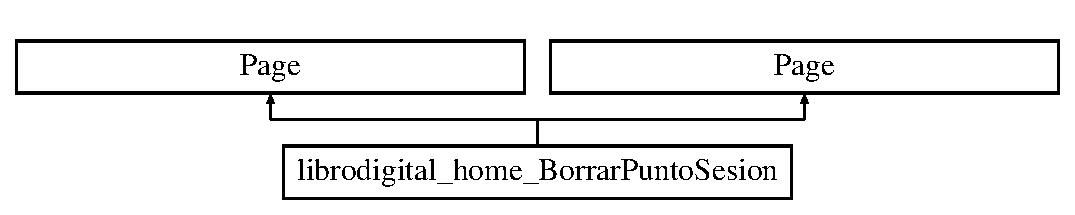
\includegraphics[height=2.000000cm]{classlibrodigital__home___borrar_punto_sesion}
\end{center}
\end{figure}
\subsection*{Protected Member Functions}
\begin{DoxyCompactItemize}
\item 
void {\bfseries Page\+\_\+\+Load} (object sender, Event\+Args e)\hypertarget{classlibrodigital__home___borrar_punto_sesion_abefe92276fd24d95ea3920f908ba7062}{}\label{classlibrodigital__home___borrar_punto_sesion_abefe92276fd24d95ea3920f908ba7062}

\item 
void {\bfseries Page\+\_\+\+Load} (object sender, Event\+Args e)\hypertarget{classlibrodigital__home___borrar_punto_sesion_abefe92276fd24d95ea3920f908ba7062}{}\label{classlibrodigital__home___borrar_punto_sesion_abefe92276fd24d95ea3920f908ba7062}

\end{DoxyCompactItemize}


\subsection{Detailed Description}


Definition at line 8 of file Borrar\+Punto\+Sesion.\+aspx.\+cs.



The documentation for this class was generated from the following files\+:\begin{DoxyCompactItemize}
\item 
home/Borrar\+Punto\+Sesion.\+aspx.\+cs\item 
home/Borrar\+Sesion.\+aspx.\+cs\end{DoxyCompactItemize}

\hypertarget{classlibrodigital__home__index}{}\section{librodigital\+\_\+home\+\_\+index Class Reference}
\label{classlibrodigital__home__index}\index{librodigital\+\_\+home\+\_\+index@{librodigital\+\_\+home\+\_\+index}}
Inheritance diagram for librodigital\+\_\+home\+\_\+index\+:\begin{figure}[H]
\begin{center}
\leavevmode
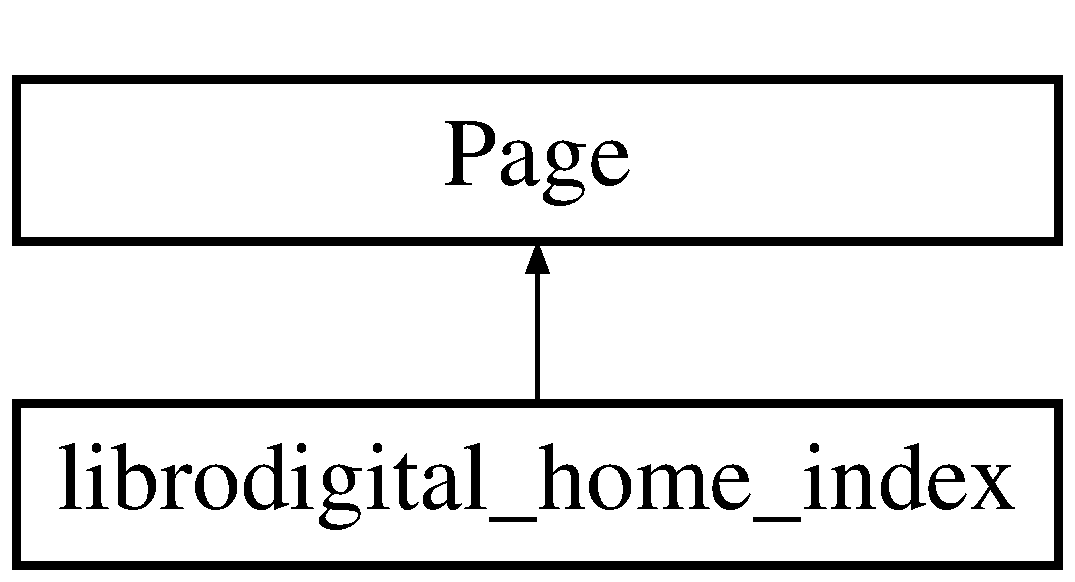
\includegraphics[height=2.000000cm]{classlibrodigital__home__index}
\end{center}
\end{figure}
\subsection*{Protected Member Functions}
\begin{DoxyCompactItemize}
\item 
void {\bfseries Page\+\_\+\+Load} (object sender, Event\+Args e)\hypertarget{classlibrodigital__home__index_a2c4adb97d3116d87066781035de7d89b}{}\label{classlibrodigital__home__index_a2c4adb97d3116d87066781035de7d89b}

\item 
void {\bfseries Button1\+\_\+\+Click} (object sender, Event\+Args e)\hypertarget{classlibrodigital__home__index_ad705566584823771f932837ca28020da}{}\label{classlibrodigital__home__index_ad705566584823771f932837ca28020da}

\end{DoxyCompactItemize}
\subsection*{Private Member Functions}
\begin{DoxyCompactItemize}
\item 
void {\bfseries Populata\+\_\+\+D\+D\+L\+\_\+anyo\+Hidrologico} ()\hypertarget{classlibrodigital__home__index_abeed0361b62df8479e6158ef902880f6}{}\label{classlibrodigital__home__index_abeed0361b62df8479e6158ef902880f6}

\item 
void {\bfseries calculos} (\hyperlink{class_sica_segura_1_1_s_i_c_a___libro_control}{Sica\+Segura.\+S\+I\+C\+A\+\_\+\+Libro\+Control} L\+CA, string FI, string FF)\hypertarget{classlibrodigital__home__index_a99d998461ab4ad42cb76ae280b4d1316}{}\label{classlibrodigital__home__index_a99d998461ab4ad42cb76ae280b4d1316}

\end{DoxyCompactItemize}
\subsection*{Private Attributes}
\begin{DoxyCompactItemize}
\item 
\hyperlink{class_sica_segura_1_1_s_i_c_a___libro_control}{Sica\+Segura.\+S\+I\+C\+A\+\_\+\+Libro\+Control} {\bfseries L\+CA}\hypertarget{classlibrodigital__home__index_a60e83fef363bb0ed461b78a3d5111bda}{}\label{classlibrodigital__home__index_a60e83fef363bb0ed461b78a3d5111bda}

\item 
Sica\+Segura.\+S\+I\+C\+A\+\_\+\+Interfaz.\+S\+I\+C\+A\+\_\+\+Libro\+Control {\bfseries Interfaz\+Libro\+Control}\hypertarget{classlibrodigital__home__index_ac3897728e36c4c51775f715dc366a8f6}{}\label{classlibrodigital__home__index_ac3897728e36c4c51775f715dc366a8f6}

\item 
Date\+Time {\bfseries FF}\hypertarget{classlibrodigital__home__index_a6e0a141827fcc2d7197ad37014c30f09}{}\label{classlibrodigital__home__index_a6e0a141827fcc2d7197ad37014c30f09}

\item 
Date\+Time {\bfseries FI}\hypertarget{classlibrodigital__home__index_a8318e0d064bb6ef05dc70200b5b10590}{}\label{classlibrodigital__home__index_a8318e0d064bb6ef05dc70200b5b10590}

\end{DoxyCompactItemize}


\subsection{Detailed Description}


Definition at line 10 of file index.\+aspx.\+cs.



The documentation for this class was generated from the following file\+:\begin{DoxyCompactItemize}
\item 
home/index.\+aspx.\+cs\end{DoxyCompactItemize}

\hypertarget{classlibrodigital__home___inf_adm}{}\section{librodigital\+\_\+home\+\_\+\+Inf\+Adm Class Reference}
\label{classlibrodigital__home___inf_adm}\index{librodigital\+\_\+home\+\_\+\+Inf\+Adm@{librodigital\+\_\+home\+\_\+\+Inf\+Adm}}
Inheritance diagram for librodigital\+\_\+home\+\_\+\+Inf\+Adm\+:\begin{figure}[H]
\begin{center}
\leavevmode
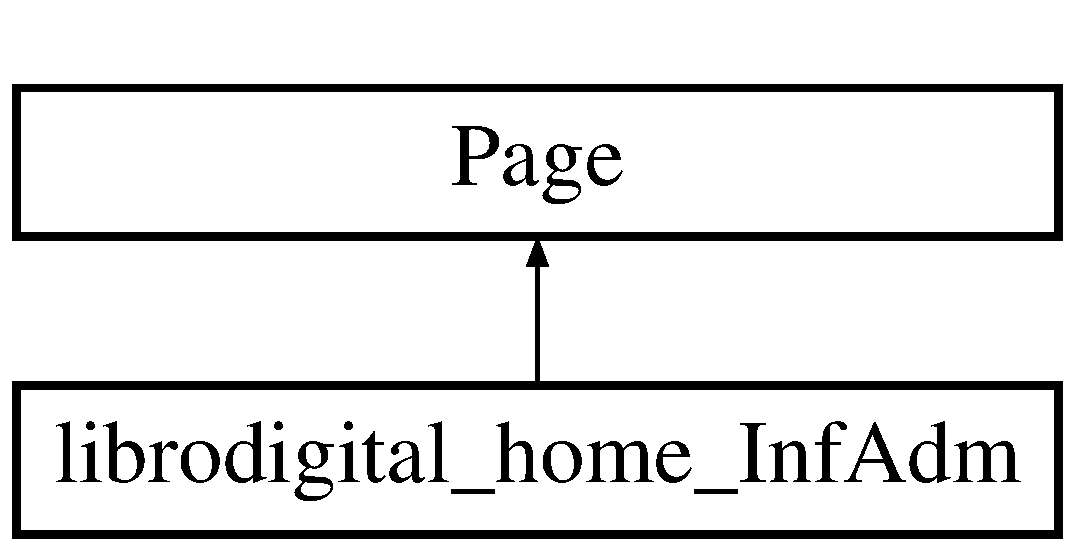
\includegraphics[height=2.000000cm]{classlibrodigital__home___inf_adm}
\end{center}
\end{figure}
\subsection*{Protected Member Functions}
\begin{DoxyCompactItemize}
\item 
void {\bfseries Page\+\_\+\+Load} (object sender, Event\+Args e)\hypertarget{classlibrodigital__home___inf_adm_a3b65a3fb2b3239ee1a7d9889e64b781b}{}\label{classlibrodigital__home___inf_adm_a3b65a3fb2b3239ee1a7d9889e64b781b}

\end{DoxyCompactItemize}
\subsection*{Private Member Functions}
\begin{DoxyCompactItemize}
\item 
void {\bfseries Muestra\+\_\+info\+\_\+\+Raacs\+\_\+formateada} (string\mbox{[}$\,$\mbox{]} campos)\hypertarget{classlibrodigital__home___inf_adm_a586a6c0d99fbc4b61f2df2082ccea1ae}{}\label{classlibrodigital__home___inf_adm_a586a6c0d99fbc4b61f2df2082ccea1ae}

\end{DoxyCompactItemize}


\subsection{Detailed Description}


Definition at line 8 of file Inf\+Adm.\+aspx.\+cs.



The documentation for this class was generated from the following file\+:\begin{DoxyCompactItemize}
\item 
home/Inf\+Adm.\+aspx.\+cs\end{DoxyCompactItemize}

\hypertarget{classlibrodigital__home___inf_geografica}{}\section{librodigital\+\_\+home\+\_\+\+Inf\+Geografica Class Reference}
\label{classlibrodigital__home___inf_geografica}\index{librodigital\+\_\+home\+\_\+\+Inf\+Geografica@{librodigital\+\_\+home\+\_\+\+Inf\+Geografica}}
Inheritance diagram for librodigital\+\_\+home\+\_\+\+Inf\+Geografica\+:\begin{figure}[H]
\begin{center}
\leavevmode
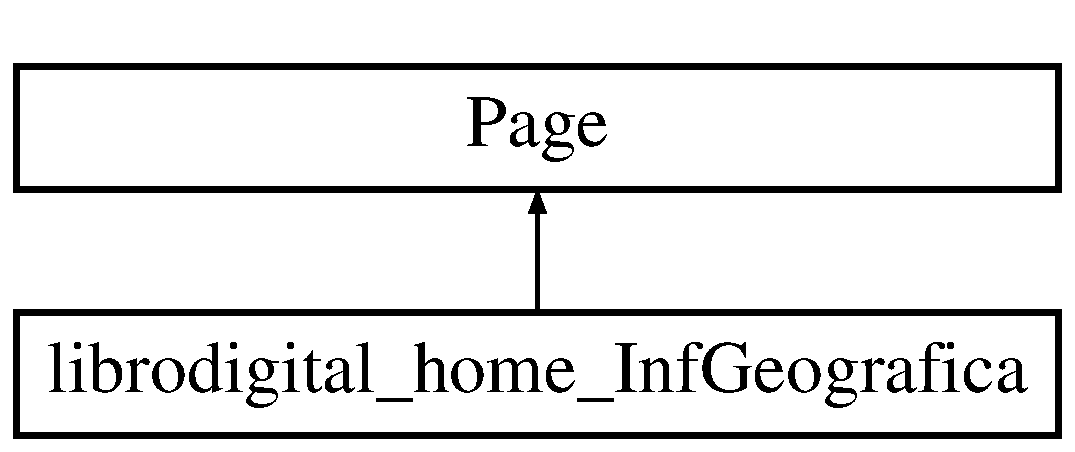
\includegraphics[height=2.000000cm]{classlibrodigital__home___inf_geografica}
\end{center}
\end{figure}
\subsection*{Protected Member Functions}
\begin{DoxyCompactItemize}
\item 
void {\bfseries Page\+\_\+\+Load} (object sender, Event\+Args e)\hypertarget{classlibrodigital__home___inf_geografica_aef99c6b4b55e673a5003cae2779cd621}{}\label{classlibrodigital__home___inf_geografica_aef99c6b4b55e673a5003cae2779cd621}

\end{DoxyCompactItemize}
\subsection*{Private Attributes}
\begin{DoxyCompactItemize}
\item 
\hyperlink{class_sica_segura_1_1_s_i_c_a___libro_control}{Sica\+Segura.\+S\+I\+C\+A\+\_\+\+Libro\+Control} {\bfseries L\+CA}\hypertarget{classlibrodigital__home___inf_geografica_a8bed2bac38863be170cfead53631e8df}{}\label{classlibrodigital__home___inf_geografica_a8bed2bac38863be170cfead53631e8df}

\item 
Sica\+Segura.\+S\+I\+C\+A\+\_\+\+Interfaz.\+S\+I\+C\+A\+\_\+\+Libro\+Control {\bfseries Interfaz\+Libro\+Control}\hypertarget{classlibrodigital__home___inf_geografica_ab3d99e7eb45c03caeb1b7c5fc31beca8}{}\label{classlibrodigital__home___inf_geografica_ab3d99e7eb45c03caeb1b7c5fc31beca8}

\end{DoxyCompactItemize}


\subsection{Detailed Description}


Definition at line 8 of file Inf\+Geografica.\+aspx.\+cs.



The documentation for this class was generated from the following file\+:\begin{DoxyCompactItemize}
\item 
home/Inf\+Geografica.\+aspx.\+cs\end{DoxyCompactItemize}

\hypertarget{classlibrodigital__home___info_usuario}{}\section{librodigital\+\_\+home\+\_\+\+Info\+Usuario Class Reference}
\label{classlibrodigital__home___info_usuario}\index{librodigital\+\_\+home\+\_\+\+Info\+Usuario@{librodigital\+\_\+home\+\_\+\+Info\+Usuario}}
Inheritance diagram for librodigital\+\_\+home\+\_\+\+Info\+Usuario\+:\begin{figure}[H]
\begin{center}
\leavevmode
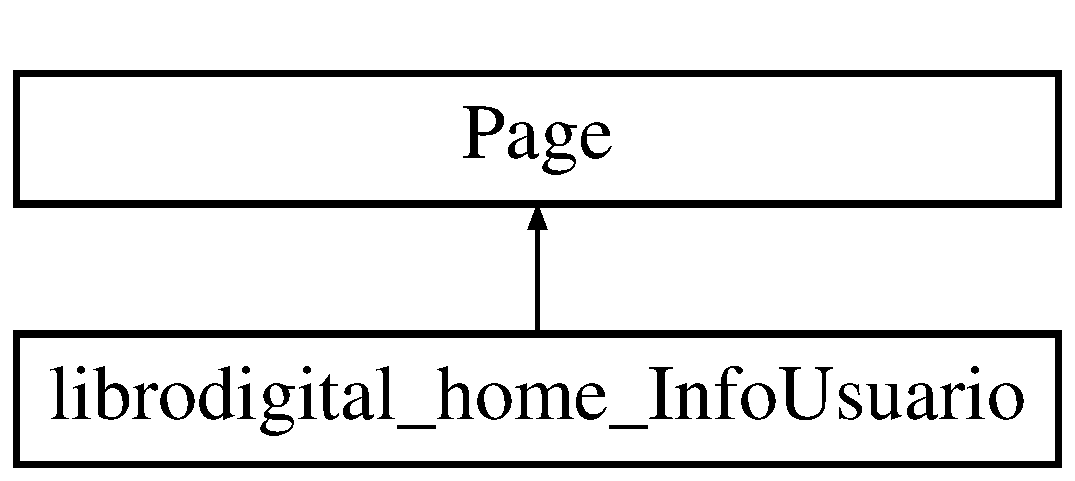
\includegraphics[height=2.000000cm]{classlibrodigital__home___info_usuario}
\end{center}
\end{figure}
\subsection*{Protected Member Functions}
\begin{DoxyCompactItemize}
\item 
void {\bfseries Page\+\_\+\+Load} (object sender, Event\+Args e)\hypertarget{classlibrodigital__home___info_usuario_a7255cbc187e4f4fbaddaef058c7b82d3}{}\label{classlibrodigital__home___info_usuario_a7255cbc187e4f4fbaddaef058c7b82d3}

\item 
void {\bfseries B\+T\+N\+\_\+\+Validar\+\_\+cambios\+\_\+\+Click} (object sender, Event\+Args e)\hypertarget{classlibrodigital__home___info_usuario_ac933430cadf2e74a72579415e76ac6c2}{}\label{classlibrodigital__home___info_usuario_ac933430cadf2e74a72579415e76ac6c2}

\end{DoxyCompactItemize}
\subsection*{Private Member Functions}
\begin{DoxyCompactItemize}
\item 
void {\bfseries Rellenar\+\_\+informacion\+\_\+contacto} (int p)\hypertarget{classlibrodigital__home___info_usuario_a48a22ade05a2abbf23077bf31a2a491e}{}\label{classlibrodigital__home___info_usuario_a48a22ade05a2abbf23077bf31a2a491e}

\end{DoxyCompactItemize}
\subsection*{Private Attributes}
\begin{DoxyCompactItemize}
\item 
\hyperlink{class_sica_segura_1_1_s_i_c_a___libro_control}{Sica\+Segura.\+S\+I\+C\+A\+\_\+\+Libro\+Control} {\bfseries L\+CA}\hypertarget{classlibrodigital__home___info_usuario_af75ca2238efad682fca81648b84a577e}{}\label{classlibrodigital__home___info_usuario_af75ca2238efad682fca81648b84a577e}

\item 
Sica\+Segura.\+S\+I\+C\+A\+\_\+\+Interfaz.\+S\+I\+C\+A\+\_\+\+Libro\+Control {\bfseries Interfaz\+Libro\+Control}\hypertarget{classlibrodigital__home___info_usuario_ad194a226993d9afcdf6685a3c38ac232}{}\label{classlibrodigital__home___info_usuario_ad194a226993d9afcdf6685a3c38ac232}

\end{DoxyCompactItemize}


\subsection{Detailed Description}


Definition at line 8 of file Info\+Usuario.\+aspx.\+cs.



The documentation for this class was generated from the following file\+:\begin{DoxyCompactItemize}
\item 
home/Info\+Usuario.\+aspx.\+cs\end{DoxyCompactItemize}

\hypertarget{classlibrodigital__home___nuevalectura}{}\section{librodigital\+\_\+home\+\_\+\+Nuevalectura Class Reference}
\label{classlibrodigital__home___nuevalectura}\index{librodigital\+\_\+home\+\_\+\+Nuevalectura@{librodigital\+\_\+home\+\_\+\+Nuevalectura}}
Inheritance diagram for librodigital\+\_\+home\+\_\+\+Nuevalectura\+:\begin{figure}[H]
\begin{center}
\leavevmode
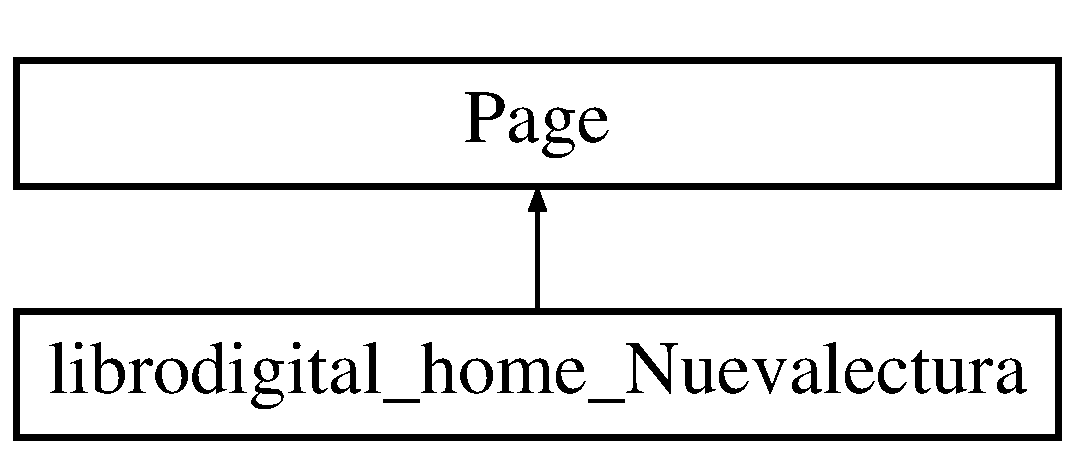
\includegraphics[height=2.000000cm]{classlibrodigital__home___nuevalectura}
\end{center}
\end{figure}
\subsection*{Protected Member Functions}
\begin{DoxyCompactItemize}
\item 
void {\bfseries Page\+\_\+\+Load} (object sender, Event\+Args e)\hypertarget{classlibrodigital__home___nuevalectura_a257b3be2eafff8690bbeff19432f9241}{}\label{classlibrodigital__home___nuevalectura_a257b3be2eafff8690bbeff19432f9241}

\end{DoxyCompactItemize}


\subsection{Detailed Description}


Definition at line 8 of file Nuevalectura.\+aspx.\+cs.



The documentation for this class was generated from the following file\+:\begin{DoxyCompactItemize}
\item 
home/Nuevalectura.\+aspx.\+cs\end{DoxyCompactItemize}

\hypertarget{class_sica_segura_1_1_s_i_c_a___agrupacion}{}\section{Sica\+Segura.\+S\+I\+C\+A\+\_\+\+Agrupacion Class Reference}
\label{class_sica_segura_1_1_s_i_c_a___agrupacion}\index{Sica\+Segura.\+S\+I\+C\+A\+\_\+\+Agrupacion@{Sica\+Segura.\+S\+I\+C\+A\+\_\+\+Agrupacion}}
\subsection*{Public Member Functions}
\begin{DoxyCompactItemize}
\item 
int {\bfseries Get\+\_\+\+Numero\+Inscripcion} ()\hypertarget{class_sica_segura_1_1_s_i_c_a___agrupacion_a09c4d394af2f286a3d182c7b373a6be8}{}\label{class_sica_segura_1_1_s_i_c_a___agrupacion_a09c4d394af2f286a3d182c7b373a6be8}

\item 
int {\bfseries Get\+\_\+\+I\+D\+Agrupacion} ()\hypertarget{class_sica_segura_1_1_s_i_c_a___agrupacion_a359ceda8d5d1bf4d5098db4ccd536e14}{}\label{class_sica_segura_1_1_s_i_c_a___agrupacion_a359ceda8d5d1bf4d5098db4ccd536e14}

\item 
double {\bfseries Get\+\_\+\+Concesion\+Inscrita} ()\hypertarget{class_sica_segura_1_1_s_i_c_a___agrupacion_a2563b37a9f8e96165a2396c40221afbc}{}\label{class_sica_segura_1_1_s_i_c_a___agrupacion_a2563b37a9f8e96165a2396c40221afbc}

\item 
double {\bfseries Get\+\_\+\+Concesion\+Modificada} ()\hypertarget{class_sica_segura_1_1_s_i_c_a___agrupacion_a6f1f88c6e030345e61fa89b9cf5f8d68}{}\label{class_sica_segura_1_1_s_i_c_a___agrupacion_a6f1f88c6e030345e61fa89b9cf5f8d68}

\item 
double {\bfseries Get\+\_\+\+Concesion\+Temporal} ()\hypertarget{class_sica_segura_1_1_s_i_c_a___agrupacion_a3b010fccb4df08e3a9168510a713ba4b}{}\label{class_sica_segura_1_1_s_i_c_a___agrupacion_a3b010fccb4df08e3a9168510a713ba4b}

\item 
double {\bfseries Get\+\_\+\+Consumido} ()\hypertarget{class_sica_segura_1_1_s_i_c_a___agrupacion_aa860531daee9cb0dee7abc0057ae05a4}{}\label{class_sica_segura_1_1_s_i_c_a___agrupacion_aa860531daee9cb0dee7abc0057ae05a4}

\item 
string\mbox{[}$\,$\mbox{]} {\bfseries Get\+\_\+\+Puntos\+De\+Contros} ()\hypertarget{class_sica_segura_1_1_s_i_c_a___agrupacion_a59a9ccb5b4d2118085fa1ce3efc8cb05}{}\label{class_sica_segura_1_1_s_i_c_a___agrupacion_a59a9ccb5b4d2118085fa1ce3efc8cb05}

\item 
string {\bfseries Get\+\_\+\+Descripcion} ()\hypertarget{class_sica_segura_1_1_s_i_c_a___agrupacion_a41b801855beb2a7ff465c12237178a0e}{}\label{class_sica_segura_1_1_s_i_c_a___agrupacion_a41b801855beb2a7ff465c12237178a0e}

\item 
bool {\bfseries Es\+Del\+Raacs} ()\hypertarget{class_sica_segura_1_1_s_i_c_a___agrupacion_a6d128a60e0dbd6fed779692affa45b9d}{}\label{class_sica_segura_1_1_s_i_c_a___agrupacion_a6d128a60e0dbd6fed779692affa45b9d}

\item 
{\bfseries S\+I\+C\+A\+\_\+\+Agrupacion} (string descripcion)\hypertarget{class_sica_segura_1_1_s_i_c_a___agrupacion_acc504dc1ba2c2d32b370108004135e74}{}\label{class_sica_segura_1_1_s_i_c_a___agrupacion_acc504dc1ba2c2d32b370108004135e74}

\item 
{\bfseries S\+I\+C\+A\+\_\+\+Agrupacion} (int inscripcion)\hypertarget{class_sica_segura_1_1_s_i_c_a___agrupacion_ac55227ea875c3e15cb424b8737b34f5f}{}\label{class_sica_segura_1_1_s_i_c_a___agrupacion_ac55227ea875c3e15cb424b8737b34f5f}

\item 
double {\bfseries Calculo\+Consumido} (int Num\+Inscripcion, Date\+Time FI, Date\+Time FF)\hypertarget{class_sica_segura_1_1_s_i_c_a___agrupacion_a10e0445d4669d6ec4fac8f2730defb67}{}\label{class_sica_segura_1_1_s_i_c_a___agrupacion_a10e0445d4669d6ec4fac8f2730defb67}

\end{DoxyCompactItemize}
\subsection*{Private Member Functions}
\begin{DoxyCompactItemize}
\item 
string {\bfseries Obtener\+Descripcion} (int Num\+Inscripcion)\hypertarget{class_sica_segura_1_1_s_i_c_a___agrupacion_aca48cdcfca7b1e05a22614c12763789b}{}\label{class_sica_segura_1_1_s_i_c_a___agrupacion_aca48cdcfca7b1e05a22614c12763789b}

\item 
void {\bfseries Get\+Id\+Agrupacion} (string descripcion)\hypertarget{class_sica_segura_1_1_s_i_c_a___agrupacion_aee9e0bab250e667510859cca1099a48b}{}\label{class_sica_segura_1_1_s_i_c_a___agrupacion_aee9e0bab250e667510859cca1099a48b}

\item 
void {\bfseries Get\+Id\+Agrupacion} (int Num\+Inscripcion)\hypertarget{class_sica_segura_1_1_s_i_c_a___agrupacion_a9ae2949f22cfabad0de6afaaaba42fe5}{}\label{class_sica_segura_1_1_s_i_c_a___agrupacion_a9ae2949f22cfabad0de6afaaaba42fe5}

\item 
double {\bfseries Obtener\+Volumen\+Inscripcion} (int Num\+Inscripcion)\hypertarget{class_sica_segura_1_1_s_i_c_a___agrupacion_ac92f985644358f261d457f9e3e392e60}{}\label{class_sica_segura_1_1_s_i_c_a___agrupacion_ac92f985644358f261d457f9e3e392e60}

\item 
double {\bfseries Obtener\+Volumen\+Modificacion\+Inscripcion} (int Num\+Inscripcion)\hypertarget{class_sica_segura_1_1_s_i_c_a___agrupacion_af27cdef8d7aa9679082b4960411b19f7}{}\label{class_sica_segura_1_1_s_i_c_a___agrupacion_af27cdef8d7aa9679082b4960411b19f7}

\item 
double {\bfseries Calculo\+Consumido} ()\hypertarget{class_sica_segura_1_1_s_i_c_a___agrupacion_a0304a161f999ad2106ad23503f5eeb91}{}\label{class_sica_segura_1_1_s_i_c_a___agrupacion_a0304a161f999ad2106ad23503f5eeb91}

\item 
string\mbox{[}$\,$\mbox{]} {\bfseries Obtener\+Listado\+Puntos} ()\hypertarget{class_sica_segura_1_1_s_i_c_a___agrupacion_acce508bfad81c4d54b47f2ffe9a547d6}{}\label{class_sica_segura_1_1_s_i_c_a___agrupacion_acce508bfad81c4d54b47f2ffe9a547d6}

\end{DoxyCompactItemize}
\subsection*{Private Attributes}
\begin{DoxyCompactItemize}
\item 
int {\bfseries Num\+Inscripcion}\hypertarget{class_sica_segura_1_1_s_i_c_a___agrupacion_ae80211ede5058324afb394264e281558}{}\label{class_sica_segura_1_1_s_i_c_a___agrupacion_ae80211ede5058324afb394264e281558}

\item 
int {\bfseries Id\+Agrupacion}\hypertarget{class_sica_segura_1_1_s_i_c_a___agrupacion_afe3a70ccfcf609ad3e919eb5d16c6a7d}{}\label{class_sica_segura_1_1_s_i_c_a___agrupacion_afe3a70ccfcf609ad3e919eb5d16c6a7d}

\item 
double {\bfseries Concesion\+\_\+inscrita}\hypertarget{class_sica_segura_1_1_s_i_c_a___agrupacion_a0b9b12ee1002ad0b83a73eab838519b8}{}\label{class_sica_segura_1_1_s_i_c_a___agrupacion_a0b9b12ee1002ad0b83a73eab838519b8}

\item 
double {\bfseries Concesion\+\_\+modificada}\hypertarget{class_sica_segura_1_1_s_i_c_a___agrupacion_af6a1547c66e6523597f8ef89d16a8945}{}\label{class_sica_segura_1_1_s_i_c_a___agrupacion_af6a1547c66e6523597f8ef89d16a8945}

\item 
double {\bfseries Modificacion\+\_\+concesion}\hypertarget{class_sica_segura_1_1_s_i_c_a___agrupacion_aa018be6ec5a90cb44d7ad272a7a6f881}{}\label{class_sica_segura_1_1_s_i_c_a___agrupacion_aa018be6ec5a90cb44d7ad272a7a6f881}

\item 
double {\bfseries Consumido}\hypertarget{class_sica_segura_1_1_s_i_c_a___agrupacion_a0bb912b4e92340bdef9c1138617493e4}{}\label{class_sica_segura_1_1_s_i_c_a___agrupacion_a0bb912b4e92340bdef9c1138617493e4}

\item 
string\mbox{[}$\,$\mbox{]} {\bfseries Puntos\+Control}\hypertarget{class_sica_segura_1_1_s_i_c_a___agrupacion_ae910cdc5e6b9ea7232e5b02507ee6edc}{}\label{class_sica_segura_1_1_s_i_c_a___agrupacion_ae910cdc5e6b9ea7232e5b02507ee6edc}

\item 
string {\bfseries Descripcion}\hypertarget{class_sica_segura_1_1_s_i_c_a___agrupacion_ae1df47e61aba464e310b36fa34b5c0f4}{}\label{class_sica_segura_1_1_s_i_c_a___agrupacion_ae1df47e61aba464e310b36fa34b5c0f4}

\item 
bool {\bfseries Raacs}\hypertarget{class_sica_segura_1_1_s_i_c_a___agrupacion_a88fe7b61505327c9c8f14cb94a6788c0}{}\label{class_sica_segura_1_1_s_i_c_a___agrupacion_a88fe7b61505327c9c8f14cb94a6788c0}

\item 
System.\+Data.\+Sql\+Client.\+Sql\+Connection {\bfseries conexion} = new System.\+Data.\+Sql\+Client.\+Sql\+Connection(Configuration\+Settings.\+App\+Settings\mbox{[}\char`\"{}dsnsegura\+\_\+migracion\char`\"{}\mbox{]})\hypertarget{class_sica_segura_1_1_s_i_c_a___agrupacion_a6160bc79c3695cba87bc9940b296e6e4}{}\label{class_sica_segura_1_1_s_i_c_a___agrupacion_a6160bc79c3695cba87bc9940b296e6e4}

\end{DoxyCompactItemize}


\subsection{Detailed Description}


Definition at line 378 of file S\+I\+C\+A\+\_\+\+Log.\+cs.



The documentation for this class was generated from the following file\+:\begin{DoxyCompactItemize}
\item 
App\+\_\+\+Code/\+C\+S\+Code/S\+I\+C\+A\+\_\+\+Log.\+cs\end{DoxyCompactItemize}

\hypertarget{class_sica_segura_1_1_s_i_c_a___d_b}{}\section{Sica\+Segura.\+S\+I\+C\+A\+\_\+\+DB Class Reference}
\label{class_sica_segura_1_1_s_i_c_a___d_b}\index{Sica\+Segura.\+S\+I\+C\+A\+\_\+\+DB@{Sica\+Segura.\+S\+I\+C\+A\+\_\+\+DB}}
\subsection*{Public Member Functions}
\begin{DoxyCompactItemize}
\item 
Data\+Table {\bfseries Get\+Data\+S\+I\+G\+V\+E\+C\+T\+OR} (string S\+QL)\hypertarget{class_sica_segura_1_1_s_i_c_a___d_b_a69dd766036eaae4e708f5ba94e4f29a0}{}\label{class_sica_segura_1_1_s_i_c_a___d_b_a69dd766036eaae4e708f5ba94e4f29a0}

\item 
Data\+Table {\bfseries Get\+Data\+D\+B\+S\+I\+CA} (string S\+QL)\hypertarget{class_sica_segura_1_1_s_i_c_a___d_b_a714e268e1ecca8f60d37c8814bf87c68}{}\label{class_sica_segura_1_1_s_i_c_a___d_b_a714e268e1ecca8f60d37c8814bf87c68}

\item 
Data\+Table {\bfseries Get\+Data\+R\+A\+A\+CS} (string S\+QL)\hypertarget{class_sica_segura_1_1_s_i_c_a___d_b_a6160cb159048c1eb1771900be646faaa}{}\label{class_sica_segura_1_1_s_i_c_a___d_b_a6160cb159048c1eb1771900be646faaa}

\item 
Data\+Set {\bfseries Get\+Data\+S\+I\+G\+V\+E\+C\+T\+O\+R\+\_\+\+DS} (string S\+QL)\hypertarget{class_sica_segura_1_1_s_i_c_a___d_b_af4276e1fdd34e5756b1af0e0284b337b}{}\label{class_sica_segura_1_1_s_i_c_a___d_b_af4276e1fdd34e5756b1af0e0284b337b}

\item 
Data\+Set {\bfseries Get\+Data\+D\+B\+S\+I\+C\+A\+\_\+\+DS} (string S\+QL)\hypertarget{class_sica_segura_1_1_s_i_c_a___d_b_a578bd73974c02cf892e4d731ca0a897f}{}\label{class_sica_segura_1_1_s_i_c_a___d_b_a578bd73974c02cf892e4d731ca0a897f}

\item 
Data\+Set {\bfseries Get\+Data\+R\+A\+A\+C\+S\+\_\+\+DS} (string S\+QL)\hypertarget{class_sica_segura_1_1_s_i_c_a___d_b_affec844b77e7b23d5bf3ec597e3c4f68}{}\label{class_sica_segura_1_1_s_i_c_a___d_b_affec844b77e7b23d5bf3ec597e3c4f68}

\end{DoxyCompactItemize}
\subsection*{Protected Member Functions}
\begin{DoxyCompactItemize}
\item 
void {\bfseries Alert} (string msg)\hypertarget{class_sica_segura_1_1_s_i_c_a___d_b_ae6261ea7cf251a75f418ea7dff1a0e62}{}\label{class_sica_segura_1_1_s_i_c_a___d_b_ae6261ea7cf251a75f418ea7dff1a0e62}

\end{DoxyCompactItemize}


\subsection{Detailed Description}


Definition at line 202 of file S\+I\+C\+A\+\_\+\+Log.\+cs.



The documentation for this class was generated from the following file\+:\begin{DoxyCompactItemize}
\item 
App\+\_\+\+Code/\+C\+S\+Code/S\+I\+C\+A\+\_\+\+Log.\+cs\end{DoxyCompactItemize}

\hypertarget{class_sica_segura_1_1_s_i_c_a___libro_control}{}\section{Sica\+Segura.\+S\+I\+C\+A\+\_\+\+Libro\+Control Class Reference}
\label{class_sica_segura_1_1_s_i_c_a___libro_control}\index{Sica\+Segura.\+S\+I\+C\+A\+\_\+\+Libro\+Control@{Sica\+Segura.\+S\+I\+C\+A\+\_\+\+Libro\+Control}}
\subsection*{Public Member Functions}
\begin{DoxyCompactItemize}
\item 
\hyperlink{class_sica_segura_1_1_s_i_c_a___libro_control_ad4df323bd4511411724db38cb1c43e0e}{S\+I\+C\+A\+\_\+\+Libro\+Control} (string usuario, string pass)
\begin{DoxyCompactList}\small\item\em Constructor que en base a los parámetros de entrada valida un usuario y crea el objeto L\+CA que contendrá toda la información aquí listada\+: ·\+Objeto Agrupación ·\+Objeto Info\+Raacs \end{DoxyCompactList}\item 
string {\bfseries Recuperar\+Info\+Raacs\+Inscripcion} ()\hypertarget{class_sica_segura_1_1_s_i_c_a___libro_control_ab6c928f999bed799c8ee00c50d902e12}{}\label{class_sica_segura_1_1_s_i_c_a___libro_control_ab6c928f999bed799c8ee00c50d902e12}

\end{DoxyCompactItemize}
\subsection*{Properties}
\begin{DoxyCompactItemize}
\item 
int {\bfseries I\+D\+\_\+\+Inscripcion}\hspace{0.3cm}{\ttfamily  \mbox{[}get, set\mbox{]}}\hypertarget{class_sica_segura_1_1_s_i_c_a___libro_control_ae5ad33a04640bb7bfdbff7a84364dc85}{}\label{class_sica_segura_1_1_s_i_c_a___libro_control_ae5ad33a04640bb7bfdbff7a84364dc85}

\item 
int {\bfseries I\+D\+\_\+usuario}\hspace{0.3cm}{\ttfamily  \mbox{[}get, set\mbox{]}}\hypertarget{class_sica_segura_1_1_s_i_c_a___libro_control_a05cd46258455ca884f0c967382a7fdeb}{}\label{class_sica_segura_1_1_s_i_c_a___libro_control_a05cd46258455ca884f0c967382a7fdeb}

\item 
bool {\bfseries Acceso\+\_\+validado}\hspace{0.3cm}{\ttfamily  \mbox{[}get, set\mbox{]}}\hypertarget{class_sica_segura_1_1_s_i_c_a___libro_control_acfbd4ea0f207ea05e7fb4b44ade26b4c}{}\label{class_sica_segura_1_1_s_i_c_a___libro_control_acfbd4ea0f207ea05e7fb4b44ade26b4c}

\item 
\hyperlink{class_sica_segura_1_1_s_i_c_a___agrupacion}{S\+I\+C\+A\+\_\+\+Agrupacion} {\bfseries Agrupacion}\hspace{0.3cm}{\ttfamily  \mbox{[}get\mbox{]}}\hypertarget{class_sica_segura_1_1_s_i_c_a___libro_control_ae30e7d9c2f9c9797f2bcec738610fd48}{}\label{class_sica_segura_1_1_s_i_c_a___libro_control_ae30e7d9c2f9c9797f2bcec738610fd48}

\end{DoxyCompactItemize}
\subsection*{Private Member Functions}
\begin{DoxyCompactItemize}
\item 
bool \hyperlink{class_sica_segura_1_1_s_i_c_a___libro_control_a88c4993cd7ff80f4e977c1f69e4db550}{validar\+\_\+acceso} (string pass)
\begin{DoxyCompactList}\small\item\em Funcion para validar el usuario y contraseña que ha sido introducido en la página de Log-\/in \end{DoxyCompactList}\item 
int \hyperlink{class_sica_segura_1_1_s_i_c_a___libro_control_a65b0d0cac67ce138a2415cab66e77b52}{Obtener\+\_\+\+I\+D\+\_\+\+Inscripcion} ()
\begin{DoxyCompactList}\small\item\em Obtencion del ID de la inscripcion en el Raacs. \end{DoxyCompactList}\end{DoxyCompactItemize}
\subsection*{Private Attributes}
\begin{DoxyCompactItemize}
\item 
string {\bfseries login}\hypertarget{class_sica_segura_1_1_s_i_c_a___libro_control_af9645429ebfabbe111e04c15a5b89b34}{}\label{class_sica_segura_1_1_s_i_c_a___libro_control_af9645429ebfabbe111e04c15a5b89b34}

\item 
int {\bfseries \+\_\+\+I\+D\+\_\+usuario}\hypertarget{class_sica_segura_1_1_s_i_c_a___libro_control_ae3c083b0d7e47c5c635f028722954544}{}\label{class_sica_segura_1_1_s_i_c_a___libro_control_ae3c083b0d7e47c5c635f028722954544}

\item 
int {\bfseries \+\_\+\+I\+D\+\_\+\+Inscripcion}\hypertarget{class_sica_segura_1_1_s_i_c_a___libro_control_a47f45eb36dab4732f7acf1ac6dedd160}{}\label{class_sica_segura_1_1_s_i_c_a___libro_control_a47f45eb36dab4732f7acf1ac6dedd160}

\item 
bool {\bfseries \+\_\+\+Acceso\+\_\+\+Validado}\hypertarget{class_sica_segura_1_1_s_i_c_a___libro_control_a0315d9f7f35d5e387afeed71c75a1462}{}\label{class_sica_segura_1_1_s_i_c_a___libro_control_a0315d9f7f35d5e387afeed71c75a1462}

\item 
\hyperlink{class_sica_segura_1_1_s_i_c_a___agrupacion}{S\+I\+C\+A\+\_\+\+Agrupacion} {\bfseries \+\_\+\+Agrupacion}\hypertarget{class_sica_segura_1_1_s_i_c_a___libro_control_a9412b76f51541edb4e117f00d4dc729f}{}\label{class_sica_segura_1_1_s_i_c_a___libro_control_a9412b76f51541edb4e117f00d4dc729f}

\item 
string {\bfseries \+\_\+\+Info\+Raacs\+\_\+splited}\hypertarget{class_sica_segura_1_1_s_i_c_a___libro_control_ac569866649fe77e5b6c87c7d3435ead5}{}\label{class_sica_segura_1_1_s_i_c_a___libro_control_ac569866649fe77e5b6c87c7d3435ead5}

\end{DoxyCompactItemize}


\subsection{Detailed Description}


Definition at line 302 of file S\+I\+C\+A\+\_\+\+Log.\+cs.



\subsection{Constructor \& Destructor Documentation}
\index{Sica\+Segura\+::\+S\+I\+C\+A\+\_\+\+Libro\+Control@{Sica\+Segura\+::\+S\+I\+C\+A\+\_\+\+Libro\+Control}!S\+I\+C\+A\+\_\+\+Libro\+Control@{S\+I\+C\+A\+\_\+\+Libro\+Control}}
\index{S\+I\+C\+A\+\_\+\+Libro\+Control@{S\+I\+C\+A\+\_\+\+Libro\+Control}!Sica\+Segura\+::\+S\+I\+C\+A\+\_\+\+Libro\+Control@{Sica\+Segura\+::\+S\+I\+C\+A\+\_\+\+Libro\+Control}}
\subsubsection[{\texorpdfstring{S\+I\+C\+A\+\_\+\+Libro\+Control(string usuario, string pass)}{SICA_LibroControl(string usuario, string pass)}}]{\setlength{\rightskip}{0pt plus 5cm}Sica\+Segura.\+S\+I\+C\+A\+\_\+\+Libro\+Control.\+S\+I\+C\+A\+\_\+\+Libro\+Control (
\begin{DoxyParamCaption}
\item[{string}]{usuario, }
\item[{string}]{pass}
\end{DoxyParamCaption}
)}\hypertarget{class_sica_segura_1_1_s_i_c_a___libro_control_ad4df323bd4511411724db38cb1c43e0e}{}\label{class_sica_segura_1_1_s_i_c_a___libro_control_ad4df323bd4511411724db38cb1c43e0e}


Constructor que en base a los parámetros de entrada valida un usuario y crea el objeto L\+CA que contendrá toda la información aquí listada\+: ·\+Objeto Agrupación ·\+Objeto Info\+Raacs 


\begin{DoxyParams}{Parameters}
{\em usuario} & Usuario a validar\\
\hline
{\em pass} & Pass a validar\\
\hline
\end{DoxyParams}


Definition at line 325 of file S\+I\+C\+A\+\_\+\+Log.\+cs.



\subsection{Member Function Documentation}
\index{Sica\+Segura\+::\+S\+I\+C\+A\+\_\+\+Libro\+Control@{Sica\+Segura\+::\+S\+I\+C\+A\+\_\+\+Libro\+Control}!Obtener\+\_\+\+I\+D\+\_\+\+Inscripcion@{Obtener\+\_\+\+I\+D\+\_\+\+Inscripcion}}
\index{Obtener\+\_\+\+I\+D\+\_\+\+Inscripcion@{Obtener\+\_\+\+I\+D\+\_\+\+Inscripcion}!Sica\+Segura\+::\+S\+I\+C\+A\+\_\+\+Libro\+Control@{Sica\+Segura\+::\+S\+I\+C\+A\+\_\+\+Libro\+Control}}
\subsubsection[{\texorpdfstring{Obtener\+\_\+\+I\+D\+\_\+\+Inscripcion()}{Obtener_ID_Inscripcion()}}]{\setlength{\rightskip}{0pt plus 5cm}int Sica\+Segura.\+S\+I\+C\+A\+\_\+\+Libro\+Control.\+Obtener\+\_\+\+I\+D\+\_\+\+Inscripcion (
\begin{DoxyParamCaption}
{}
\end{DoxyParamCaption}
)\hspace{0.3cm}{\ttfamily [private]}}\hypertarget{class_sica_segura_1_1_s_i_c_a___libro_control_a65b0d0cac67ce138a2415cab66e77b52}{}\label{class_sica_segura_1_1_s_i_c_a___libro_control_a65b0d0cac67ce138a2415cab66e77b52}


Obtencion del ID de la inscripcion en el Raacs. 

\begin{DoxyReturn}{Returns}
Devuelve un valor entero que corresponde con el Nº de inscripción
\end{DoxyReturn}


Definition at line 351 of file S\+I\+C\+A\+\_\+\+Log.\+cs.

\index{Sica\+Segura\+::\+S\+I\+C\+A\+\_\+\+Libro\+Control@{Sica\+Segura\+::\+S\+I\+C\+A\+\_\+\+Libro\+Control}!validar\+\_\+acceso@{validar\+\_\+acceso}}
\index{validar\+\_\+acceso@{validar\+\_\+acceso}!Sica\+Segura\+::\+S\+I\+C\+A\+\_\+\+Libro\+Control@{Sica\+Segura\+::\+S\+I\+C\+A\+\_\+\+Libro\+Control}}
\subsubsection[{\texorpdfstring{validar\+\_\+acceso(string pass)}{validar_acceso(string pass)}}]{\setlength{\rightskip}{0pt plus 5cm}bool Sica\+Segura.\+S\+I\+C\+A\+\_\+\+Libro\+Control.\+validar\+\_\+acceso (
\begin{DoxyParamCaption}
\item[{string}]{pass}
\end{DoxyParamCaption}
)\hspace{0.3cm}{\ttfamily [private]}}\hypertarget{class_sica_segura_1_1_s_i_c_a___libro_control_a88c4993cd7ff80f4e977c1f69e4db550}{}\label{class_sica_segura_1_1_s_i_c_a___libro_control_a88c4993cd7ff80f4e977c1f69e4db550}


Funcion para validar el usuario y contraseña que ha sido introducido en la página de Log-\/in 


\begin{DoxyParams}{Parameters}
{\em pass} & Parametro que contiene la contraseña del usuario\\
\hline
\end{DoxyParams}
\begin{DoxyReturn}{Returns}
Un valor Booleano
\end{DoxyReturn}


Definition at line 341 of file S\+I\+C\+A\+\_\+\+Log.\+cs.



The documentation for this class was generated from the following file\+:\begin{DoxyCompactItemize}
\item 
App\+\_\+\+Code/\+C\+S\+Code/S\+I\+C\+A\+\_\+\+Log.\+cs\end{DoxyCompactItemize}

\hypertarget{class_sica_segura_1_1_s_i_c_a___log}{}\section{Sica\+Segura.\+S\+I\+C\+A\+\_\+\+Log Class Reference}
\label{class_sica_segura_1_1_s_i_c_a___log}\index{Sica\+Segura.\+S\+I\+C\+A\+\_\+\+Log@{Sica\+Segura.\+S\+I\+C\+A\+\_\+\+Log}}


Clase cuya función es la de registrar los movimientos realizados en la Web.  


\subsection*{Public Member Functions}
\begin{DoxyCompactItemize}
\item 
void {\bfseries acceso\+\_\+pagina} ()\hypertarget{class_sica_segura_1_1_s_i_c_a___log_a7bb312304ee61c899f4e95f10d11a699}{}\label{class_sica_segura_1_1_s_i_c_a___log_a7bb312304ee61c899f4e95f10d11a699}

\item 
void {\bfseries acceso\+\_\+\+Cauces\+\_\+y\+\_\+puntos} ()\hypertarget{class_sica_segura_1_1_s_i_c_a___log_a703b1e54d8b837cbc0a00a55209b9f6d}{}\label{class_sica_segura_1_1_s_i_c_a___log_a703b1e54d8b837cbc0a00a55209b9f6d}

\item 
void {\bfseries acceso\+\_\+\+Mantenimientos} ()\hypertarget{class_sica_segura_1_1_s_i_c_a___log_a46d4ec9c82a9a1e32092d35803141475}{}\label{class_sica_segura_1_1_s_i_c_a___log_a46d4ec9c82a9a1e32092d35803141475}

\item 
void {\bfseries acceso\+\_\+\+Mantenimientos\+\_\+cauces} ()\hypertarget{class_sica_segura_1_1_s_i_c_a___log_a75f29e26508ba314e6e87d8a5f48eeb7}{}\label{class_sica_segura_1_1_s_i_c_a___log_a75f29e26508ba314e6e87d8a5f48eeb7}

\item 
void {\bfseries Alta\+\_\+\+Mantenimientos\+\_\+cauces} ()\hypertarget{class_sica_segura_1_1_s_i_c_a___log_a4b2f01844d9bbe383c69fdfb7bca6e55}{}\label{class_sica_segura_1_1_s_i_c_a___log_a4b2f01844d9bbe383c69fdfb7bca6e55}

\item 
void {\bfseries Modificacion\+\_\+\+Mantenimientos\+\_\+cauces} ()\hypertarget{class_sica_segura_1_1_s_i_c_a___log_afb7026c39112be6b6ec4d9de55114876}{}\label{class_sica_segura_1_1_s_i_c_a___log_afb7026c39112be6b6ec4d9de55114876}

\item 
void {\bfseries acceso\+\_\+\+Mantenimientos\+\_\+puntos} ()\hypertarget{class_sica_segura_1_1_s_i_c_a___log_aa2cdb2a9b132b38b08189d65f66b2fde}{}\label{class_sica_segura_1_1_s_i_c_a___log_aa2cdb2a9b132b38b08189d65f66b2fde}

\item 
void {\bfseries Alta\+\_\+\+Mantenimientos\+\_\+puntos} ()\hypertarget{class_sica_segura_1_1_s_i_c_a___log_ac6ae4dbf27bb374d29b4e1e5fa6015e8}{}\label{class_sica_segura_1_1_s_i_c_a___log_ac6ae4dbf27bb374d29b4e1e5fa6015e8}

\item 
void {\bfseries Modificacion\+\_\+\+Mantenimientos\+\_\+puntos} ()\hypertarget{class_sica_segura_1_1_s_i_c_a___log_a6c4c8ee804e21b0b0f77fea076bfb0af}{}\label{class_sica_segura_1_1_s_i_c_a___log_a6c4c8ee804e21b0b0f77fea076bfb0af}

\item 
void {\bfseries acceso\+\_\+\+Mantenimientos\+\_\+\+Elemento\+Medida} ()\hypertarget{class_sica_segura_1_1_s_i_c_a___log_a6a665e9347903784a427aca1d1318d90}{}\label{class_sica_segura_1_1_s_i_c_a___log_a6a665e9347903784a427aca1d1318d90}

\item 
void {\bfseries Alta\+\_\+\+Mantenimientos\+\_\+\+Elemento\+Medida} ()\hypertarget{class_sica_segura_1_1_s_i_c_a___log_a4c1d1bde96fee0c24cd612cd3d2e8d4e}{}\label{class_sica_segura_1_1_s_i_c_a___log_a4c1d1bde96fee0c24cd612cd3d2e8d4e}

\item 
void {\bfseries Modificacion\+\_\+\+Mantenimientos\+\_\+\+Elemento\+Medida} ()\hypertarget{class_sica_segura_1_1_s_i_c_a___log_a3f0634dc6e01b9aa35f33268650fd56d}{}\label{class_sica_segura_1_1_s_i_c_a___log_a3f0634dc6e01b9aa35f33268650fd56d}

\item 
void {\bfseries Borrado\+\_\+\+Mantenimientos\+\_\+\+Elemento\+Medida} ()\hypertarget{class_sica_segura_1_1_s_i_c_a___log_aba62e16c4d4d2bdb89d2468e4f649dfd}{}\label{class_sica_segura_1_1_s_i_c_a___log_aba62e16c4d4d2bdb89d2468e4f649dfd}

\item 
void {\bfseries Acceso\+\_\+\+Mantenimientos\+\_\+curvas} ()\hypertarget{class_sica_segura_1_1_s_i_c_a___log_a5676b014ff43688bf63640717b175e2f}{}\label{class_sica_segura_1_1_s_i_c_a___log_a5676b014ff43688bf63640717b175e2f}

\item 
void {\bfseries Alta\+\_\+\+Mantenimientos\+\_\+curvas} ()\hypertarget{class_sica_segura_1_1_s_i_c_a___log_a63d22418c1159aae360a1c2e9f1068c2}{}\label{class_sica_segura_1_1_s_i_c_a___log_a63d22418c1159aae360a1c2e9f1068c2}

\item 
void {\bfseries Modificacion\+\_\+\+Mantenimientos\+\_\+curvas} ()\hypertarget{class_sica_segura_1_1_s_i_c_a___log_a2f1b905e28a3582dc3b29a1ca01f1a53}{}\label{class_sica_segura_1_1_s_i_c_a___log_a2f1b905e28a3582dc3b29a1ca01f1a53}

\item 
void {\bfseries Borrado\+\_\+\+Mantenimientos\+\_\+curvas} ()\hypertarget{class_sica_segura_1_1_s_i_c_a___log_aa9f3a315f49bc14770f511a763fabf54}{}\label{class_sica_segura_1_1_s_i_c_a___log_aa9f3a315f49bc14770f511a763fabf54}

\item 
void {\bfseries acceso\+\_\+\+Mantenimientos\+\_\+boletines} ()\hypertarget{class_sica_segura_1_1_s_i_c_a___log_afcfe9999baebb9b53946816af08f1afa}{}\label{class_sica_segura_1_1_s_i_c_a___log_afcfe9999baebb9b53946816af08f1afa}

\item 
void {\bfseries Alta\+\_\+\+Mantenimientos\+\_\+boletines} ()\hypertarget{class_sica_segura_1_1_s_i_c_a___log_a5990e28621a5f04d0f096841f4ab5c97}{}\label{class_sica_segura_1_1_s_i_c_a___log_a5990e28621a5f04d0f096841f4ab5c97}

\item 
void {\bfseries Modificacion\+\_\+\+Mantenimientos\+\_\+boletines} ()\hypertarget{class_sica_segura_1_1_s_i_c_a___log_a6fdd9f85d55a128a40d1bed6c858b00f}{}\label{class_sica_segura_1_1_s_i_c_a___log_a6fdd9f85d55a128a40d1bed6c858b00f}

\item 
void {\bfseries Borrado\+\_\+\+Mantenimientos\+\_\+boletines} ()\hypertarget{class_sica_segura_1_1_s_i_c_a___log_a26261b89361c0459534b3fc62f7c7bed}{}\label{class_sica_segura_1_1_s_i_c_a___log_a26261b89361c0459534b3fc62f7c7bed}

\item 
void {\bfseries acceso\+\_\+\+Mantenimientos\+\_\+\+Seguimiento} ()\hypertarget{class_sica_segura_1_1_s_i_c_a___log_a980c86e2b5c4c81a67fdc635bd712c6d}{}\label{class_sica_segura_1_1_s_i_c_a___log_a980c86e2b5c4c81a67fdc635bd712c6d}

\item 
void {\bfseries Alta\+\_\+\+Mantenimientos\+\_\+\+Seguimiento} ()\hypertarget{class_sica_segura_1_1_s_i_c_a___log_adae5d9238f03469b070a99edc4c1ed40}{}\label{class_sica_segura_1_1_s_i_c_a___log_adae5d9238f03469b070a99edc4c1ed40}

\item 
void {\bfseries Modificacion\+\_\+\+Mantenimientos\+\_\+\+Seguimiento} ()\hypertarget{class_sica_segura_1_1_s_i_c_a___log_aa9adea4bd2afc0c6d21659607aced1f7}{}\label{class_sica_segura_1_1_s_i_c_a___log_aa9adea4bd2afc0c6d21659607aced1f7}

\item 
void {\bfseries Borrado\+\_\+\+Mantenimientos\+\_\+\+Seguimiento} ()\hypertarget{class_sica_segura_1_1_s_i_c_a___log_aaf8e68471a47338df181bf30fed33f09}{}\label{class_sica_segura_1_1_s_i_c_a___log_aaf8e68471a47338df181bf30fed33f09}

\item 
void {\bfseries Acceso\+\_\+\+S\+CV} (string url)\hypertarget{class_sica_segura_1_1_s_i_c_a___log_ac6a73b8bb762030cdd5554fb19fdb09d}{}\label{class_sica_segura_1_1_s_i_c_a___log_ac6a73b8bb762030cdd5554fb19fdb09d}

\item 
void {\bfseries Descarga\+\_\+\+S\+C\+V\+\_\+\+Alberca\+\_\+informe} ()\hypertarget{class_sica_segura_1_1_s_i_c_a___log_acbab781b6fc7be744c75a3831e31ac38}{}\label{class_sica_segura_1_1_s_i_c_a___log_acbab781b6fc7be744c75a3831e31ac38}

\item 
void {\bfseries Acceso\+\_\+\+S\+C\+V\+\_\+\+R\+A\+A\+CS} ()\hypertarget{class_sica_segura_1_1_s_i_c_a___log_a6e0bdd6616b400331e0046b2d39c798f}{}\label{class_sica_segura_1_1_s_i_c_a___log_a6e0bdd6616b400331e0046b2d39c798f}

\item 
void {\bfseries Descarga\+\_\+\+S\+C\+V\+\_\+\+R\+A\+A\+C\+S\+\_\+informe} ()\hypertarget{class_sica_segura_1_1_s_i_c_a___log_a2c27d65ce8c5358a7a6e08b0c6e815d3}{}\label{class_sica_segura_1_1_s_i_c_a___log_a2c27d65ce8c5358a7a6e08b0c6e815d3}

\item 
void {\bfseries Acceso\+\_\+\+S\+C\+V\+\_\+\+S\+I\+CA} ()\hypertarget{class_sica_segura_1_1_s_i_c_a___log_a9e2342c5c1e9a0e8c25ea845bd7c4621}{}\label{class_sica_segura_1_1_s_i_c_a___log_a9e2342c5c1e9a0e8c25ea845bd7c4621}

\item 
void {\bfseries Descarga\+\_\+\+S\+C\+V\+\_\+\+S\+I\+C\+A\+\_\+informe} (string concepto)\hypertarget{class_sica_segura_1_1_s_i_c_a___log_acc474b43cdee0cc1ea2462aa100a551e}{}\label{class_sica_segura_1_1_s_i_c_a___log_acc474b43cdee0cc1ea2462aa100a551e}

\end{DoxyCompactItemize}
\subsection*{Private Attributes}
\begin{DoxyCompactItemize}
\item 
Sql\+Connection {\bfseries conn}\hypertarget{class_sica_segura_1_1_s_i_c_a___log_a53b3b913dbf6cbf7d5104ec1ba16d977}{}\label{class_sica_segura_1_1_s_i_c_a___log_a53b3b913dbf6cbf7d5104ec1ba16d977}

\end{DoxyCompactItemize}


\subsection{Detailed Description}
Clase cuya función es la de registrar los movimientos realizados en la Web. 



Definition at line 15 of file S\+I\+C\+A\+\_\+\+Log.\+cs.



The documentation for this class was generated from the following file\+:\begin{DoxyCompactItemize}
\item 
App\+\_\+\+Code/\+C\+S\+Code/S\+I\+C\+A\+\_\+\+Log.\+cs\end{DoxyCompactItemize}

\hypertarget{class_sica_segura_1_1_s_i_c_a___punto_control}{}\section{Sica\+Segura.\+S\+I\+C\+A\+\_\+\+Punto\+Control Class Reference}
\label{class_sica_segura_1_1_s_i_c_a___punto_control}\index{Sica\+Segura.\+S\+I\+C\+A\+\_\+\+Punto\+Control@{Sica\+Segura.\+S\+I\+C\+A\+\_\+\+Punto\+Control}}
\subsection*{Classes}
\begin{DoxyCompactItemize}
\item 
class \hyperlink{class_sica_segura_1_1_s_i_c_a___punto_control_1_1_lectura}{Lectura}
\end{DoxyCompactItemize}
\subsection*{Public Member Functions}
\begin{DoxyCompactItemize}
\item 
{\bfseries S\+I\+C\+A\+\_\+\+Punto\+Control} (string Pvycr)\hypertarget{class_sica_segura_1_1_s_i_c_a___punto_control_a7e613b7627400d4fcd71c0c149a38c79}{}\label{class_sica_segura_1_1_s_i_c_a___punto_control_a7e613b7627400d4fcd71c0c149a38c79}

\item 
double {\bfseries Consumo\+Por\+Volumetrico} (Date\+Time FI, Date\+Time FF)\hypertarget{class_sica_segura_1_1_s_i_c_a___punto_control_a7ccf6a66a7157e7992b145d513b536ce}{}\label{class_sica_segura_1_1_s_i_c_a___punto_control_a7ccf6a66a7157e7992b145d513b536ce}

\item 
double {\bfseries Consumo\+Por\+Caudalimetro} (Date\+Time FI, Date\+Time FF)\hypertarget{class_sica_segura_1_1_s_i_c_a___punto_control_af858df6bcbbd0e608b20591989f232ce}{}\label{class_sica_segura_1_1_s_i_c_a___punto_control_af858df6bcbbd0e608b20591989f232ce}

\item 
double {\bfseries Consumo\+Por\+Electrico} (Date\+Time FI, Date\+Time FF)\hypertarget{class_sica_segura_1_1_s_i_c_a___punto_control_a131e0fea599607032ed64aa23fe6f024}{}\label{class_sica_segura_1_1_s_i_c_a___punto_control_a131e0fea599607032ed64aa23fe6f024}

\item 
double {\bfseries Consumo\+Por\+Horometro} (Date\+Time FI, Date\+Time FF)\hypertarget{class_sica_segura_1_1_s_i_c_a___punto_control_ab7f245c76354534c07715e53c92f9dc0}{}\label{class_sica_segura_1_1_s_i_c_a___punto_control_ab7f245c76354534c07715e53c92f9dc0}

\end{DoxyCompactItemize}
\subsection*{Private Member Functions}
\begin{DoxyCompactItemize}
\item 
void {\bfseries Obtener\+EM} ()\hypertarget{class_sica_segura_1_1_s_i_c_a___punto_control_aeaec7c94240d1e8d67ba0cb5fb92eac5}{}\label{class_sica_segura_1_1_s_i_c_a___punto_control_aeaec7c94240d1e8d67ba0cb5fb92eac5}

\item 
\hyperlink{class_sica_segura_1_1_s_i_c_a___punto_control_1_1_lectura}{Lectura} {\bfseries Interpolar\+Lecturas} (\hyperlink{class_sica_segura_1_1_s_i_c_a___punto_control_1_1_lectura}{Lectura} Lec\+Prev, \hyperlink{class_sica_segura_1_1_s_i_c_a___punto_control_1_1_lectura}{Lectura} Lec\+Post, Date\+Time fecha\+A\+Interpolar)\hypertarget{class_sica_segura_1_1_s_i_c_a___punto_control_a8fe23db24b380334aae093374f59a828}{}\label{class_sica_segura_1_1_s_i_c_a___punto_control_a8fe23db24b380334aae093374f59a828}

\item 
\hyperlink{class_sica_segura_1_1_s_i_c_a___punto_control_1_1_lectura}{Lectura} {\bfseries Obtener\+\_\+\+Lectura\+\_\+volumetrica\+\_\+\+Anterior} (Date\+Time Fecha)\hypertarget{class_sica_segura_1_1_s_i_c_a___punto_control_ade125def28d40a3bfe6039cc6a2a6310}{}\label{class_sica_segura_1_1_s_i_c_a___punto_control_ade125def28d40a3bfe6039cc6a2a6310}

\item 
\hyperlink{class_sica_segura_1_1_s_i_c_a___punto_control_1_1_lectura}{Lectura} {\bfseries Obtener\+\_\+\+Lectura\+\_\+volumetrica\+\_\+\+Posterior} (Date\+Time Fecha)\hypertarget{class_sica_segura_1_1_s_i_c_a___punto_control_a0c0929ba6efda438e6040c1ddb983477}{}\label{class_sica_segura_1_1_s_i_c_a___punto_control_a0c0929ba6efda438e6040c1ddb983477}

\end{DoxyCompactItemize}
\subsection*{Private Attributes}
\begin{DoxyCompactItemize}
\item 
string {\bfseries codigo\+P\+V\+Y\+CR}\hypertarget{class_sica_segura_1_1_s_i_c_a___punto_control_aafab8ca2eb83a4e68d43f9d2b74c19fb}{}\label{class_sica_segura_1_1_s_i_c_a___punto_control_aafab8ca2eb83a4e68d43f9d2b74c19fb}

\item 
string\mbox{[}$\,$\mbox{]} {\bfseries Elementos\+De\+Medida}\hypertarget{class_sica_segura_1_1_s_i_c_a___punto_control_a63435f1782ec77457312fd6576875011}{}\label{class_sica_segura_1_1_s_i_c_a___punto_control_a63435f1782ec77457312fd6576875011}

\end{DoxyCompactItemize}


\subsection{Detailed Description}


Definition at line 609 of file S\+I\+C\+A\+\_\+\+Log.\+cs.



The documentation for this class was generated from the following file\+:\begin{DoxyCompactItemize}
\item 
App\+\_\+\+Code/\+C\+S\+Code/S\+I\+C\+A\+\_\+\+Log.\+cs\end{DoxyCompactItemize}

\hypertarget{class_sica_segura_1_1_s_i_c_a___sysem_i_o}{}\section{Sica\+Segura.\+S\+I\+C\+A\+\_\+\+Sysem\+IO Class Reference}
\label{class_sica_segura_1_1_s_i_c_a___sysem_i_o}\index{Sica\+Segura.\+S\+I\+C\+A\+\_\+\+Sysem\+IO@{Sica\+Segura.\+S\+I\+C\+A\+\_\+\+Sysem\+IO}}
\subsection*{Public Member Functions}
\begin{DoxyCompactItemize}
\item 
bool {\bfseries Existe\+Carpeta\+En\+Servidor} (string carpeta)\hypertarget{class_sica_segura_1_1_s_i_c_a___sysem_i_o_af852b64186eb239ff9d08b9734a1f569}{}\label{class_sica_segura_1_1_s_i_c_a___sysem_i_o_af852b64186eb239ff9d08b9734a1f569}

\end{DoxyCompactItemize}


\subsection{Detailed Description}


Definition at line 699 of file S\+I\+C\+A\+\_\+\+Log.\+cs.



The documentation for this class was generated from the following file\+:\begin{DoxyCompactItemize}
\item 
App\+\_\+\+Code/\+C\+S\+Code/S\+I\+C\+A\+\_\+\+Log.\+cs\end{DoxyCompactItemize}

\hypertarget{class_s_i_c_a_h___galeria__galeria}{}\section{S\+I\+C\+A\+H\+\_\+\+Galeria\+\_\+galeria Class Reference}
\label{class_s_i_c_a_h___galeria__galeria}\index{S\+I\+C\+A\+H\+\_\+\+Galeria\+\_\+galeria@{S\+I\+C\+A\+H\+\_\+\+Galeria\+\_\+galeria}}
Inheritance diagram for S\+I\+C\+A\+H\+\_\+\+Galeria\+\_\+galeria\+:\begin{figure}[H]
\begin{center}
\leavevmode
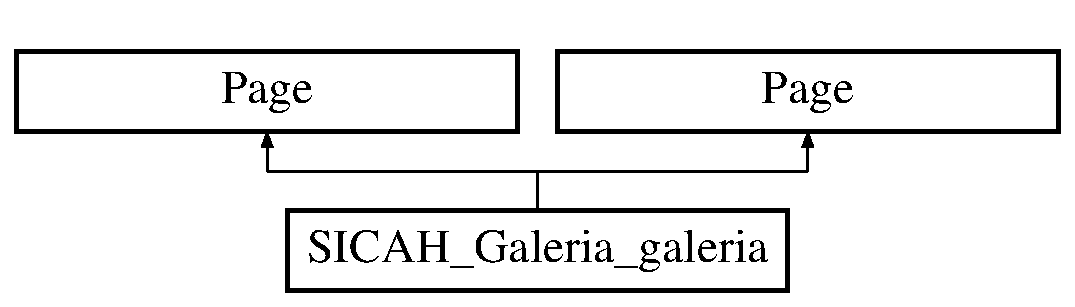
\includegraphics[height=2.000000cm]{class_s_i_c_a_h___galeria__galeria}
\end{center}
\end{figure}
\subsection*{Protected Member Functions}
\begin{DoxyCompactItemize}
\item 
void {\bfseries Page\+\_\+\+Load} (object sender, Event\+Args e)\hypertarget{class_s_i_c_a_h___galeria__galeria_ae5d0b13c17e9bd507dbbe74e30e8bd45}{}\label{class_s_i_c_a_h___galeria__galeria_ae5d0b13c17e9bd507dbbe74e30e8bd45}

\item 
void {\bfseries Page\+\_\+\+Load} (object sender, Event\+Args e)\hypertarget{class_s_i_c_a_h___galeria__galeria_ae5d0b13c17e9bd507dbbe74e30e8bd45}{}\label{class_s_i_c_a_h___galeria__galeria_ae5d0b13c17e9bd507dbbe74e30e8bd45}

\end{DoxyCompactItemize}
\subsection*{Private Member Functions}
\begin{DoxyCompactItemize}
\item 
string {\bfseries get\+\_\+listado\+Puntos\+Menu\+Lateral\+Esquemas} ()\hypertarget{class_s_i_c_a_h___galeria__galeria_a40a729dcfc611d424a4ff712fa6d663c}{}\label{class_s_i_c_a_h___galeria__galeria_a40a729dcfc611d424a4ff712fa6d663c}

\item 
void {\bfseries comprobar\+Thumbails} ()\hypertarget{class_s_i_c_a_h___galeria__galeria_a935d122fb188bc13e60d3a74ea87f47d}{}\label{class_s_i_c_a_h___galeria__galeria_a935d122fb188bc13e60d3a74ea87f47d}

\item 
void {\bfseries Prepara\+Thumbails\+Dir} ()\hypertarget{class_s_i_c_a_h___galeria__galeria_ac8aadd8d535b52d8e2117560cd5803b1}{}\label{class_s_i_c_a_h___galeria__galeria_ac8aadd8d535b52d8e2117560cd5803b1}

\item 
void {\bfseries Generate\+Thumb\+Nail} (string sourcefile, string destinationfile, int width)\hypertarget{class_s_i_c_a_h___galeria__galeria_a29c1269960bdd71448aab3bc51b4ee68}{}\label{class_s_i_c_a_h___galeria__galeria_a29c1269960bdd71448aab3bc51b4ee68}

\item 
void {\bfseries configurar\+Pagina} ()\hypertarget{class_s_i_c_a_h___galeria__galeria_a5dce90bf1628bf8a761875eab63869d3}{}\label{class_s_i_c_a_h___galeria__galeria_a5dce90bf1628bf8a761875eab63869d3}

\item 
void {\bfseries Generar\+Croquis} ()\hypertarget{class_s_i_c_a_h___galeria__galeria_a8d25c739551a131344b0382f610cd429}{}\label{class_s_i_c_a_h___galeria__galeria_a8d25c739551a131344b0382f610cd429}

\item 
string {\bfseries get\+\_\+listado\+Puntos\+Menu\+Lateral\+Fotos} ()\hypertarget{class_s_i_c_a_h___galeria__galeria_a9be3c074de302e7917bf6598df4a0da5}{}\label{class_s_i_c_a_h___galeria__galeria_a9be3c074de302e7917bf6598df4a0da5}

\item 
void {\bfseries comprobar\+Thumbails} ()\hypertarget{class_s_i_c_a_h___galeria__galeria_a935d122fb188bc13e60d3a74ea87f47d}{}\label{class_s_i_c_a_h___galeria__galeria_a935d122fb188bc13e60d3a74ea87f47d}

\item 
void {\bfseries Prepara\+Thumbails\+Dir} ()\hypertarget{class_s_i_c_a_h___galeria__galeria_ac8aadd8d535b52d8e2117560cd5803b1}{}\label{class_s_i_c_a_h___galeria__galeria_ac8aadd8d535b52d8e2117560cd5803b1}

\item 
void {\bfseries Generate\+Thumb\+Nail} (string sourcefile, string destinationfile, int width)\hypertarget{class_s_i_c_a_h___galeria__galeria_a29c1269960bdd71448aab3bc51b4ee68}{}\label{class_s_i_c_a_h___galeria__galeria_a29c1269960bdd71448aab3bc51b4ee68}

\item 
void {\bfseries configurar\+Pagina} ()\hypertarget{class_s_i_c_a_h___galeria__galeria_a5dce90bf1628bf8a761875eab63869d3}{}\label{class_s_i_c_a_h___galeria__galeria_a5dce90bf1628bf8a761875eab63869d3}

\item 
void {\bfseries Generar\+Croquis} ()\hypertarget{class_s_i_c_a_h___galeria__galeria_a8d25c739551a131344b0382f610cd429}{}\label{class_s_i_c_a_h___galeria__galeria_a8d25c739551a131344b0382f610cd429}

\end{DoxyCompactItemize}
\subsection*{Private Attributes}
\begin{DoxyCompactItemize}
\item 
\hyperlink{class_sica_segura_1_1_s_i_c_a___libro_control}{Sica\+Segura.\+S\+I\+C\+A\+\_\+\+Libro\+Control} {\bfseries L\+CA}\hypertarget{class_s_i_c_a_h___galeria__galeria_ae052d69fa1668ee037b82654155b462f}{}\label{class_s_i_c_a_h___galeria__galeria_ae052d69fa1668ee037b82654155b462f}

\item 
Sica\+Segura.\+S\+I\+C\+A\+\_\+\+Interfaz.\+S\+I\+C\+A\+\_\+\+Libro\+Control {\bfseries Interfaz\+Libro\+Control}\hypertarget{class_s_i_c_a_h___galeria__galeria_a49bda3dd97288c7ba28604295a8d7f6e}{}\label{class_s_i_c_a_h___galeria__galeria_a49bda3dd97288c7ba28604295a8d7f6e}

\item 
string {\bfseries pvycr} = \char`\"{}\char`\"{}\hypertarget{class_s_i_c_a_h___galeria__galeria_a63395fa9b80ed0a156ba13e15f949ef2}{}\label{class_s_i_c_a_h___galeria__galeria_a63395fa9b80ed0a156ba13e15f949ef2}

\item 
string {\bfseries Dirbase} =\char`\"{}C\+:\textbackslash{}\textbackslash{}\+Inetpub\textbackslash{}\textbackslash{}wwwroot\textbackslash{}\textbackslash{}\+Base\+Fotografica\textbackslash{}\textbackslash{}\+Images\textbackslash{}\textbackslash{}01-\/Croquis\char`\"{}\hypertarget{class_s_i_c_a_h___galeria__galeria_a11713d69252798356446d7956e115597}{}\label{class_s_i_c_a_h___galeria__galeria_a11713d69252798356446d7956e115597}

\end{DoxyCompactItemize}


\subsection{Detailed Description}


Definition at line 11 of file esquemas.\+aspx.\+cs.



The documentation for this class was generated from the following files\+:\begin{DoxyCompactItemize}
\item 
home/esquemas.\+aspx.\+cs\item 
home/galeria.\+aspx.\+cs\end{DoxyCompactItemize}

%--- End generated contents ---

% Index
\backmatter
\newpage
\phantomsection
\clearemptydoublepage
\addcontentsline{toc}{chapter}{Index}
\printindex

\end{document}
